%&latex
\documentclass[12pt]{article}
\usepackage{amsmath}
\usepackage{graphicx,psfrag,epsf}
\usepackage{enumerate}
\usepackage{natbib}
\usepackage{url} % not crucial - just used below for the URL 

\usepackage{amssymb, qtree, bm, multirow, textcmds, siunitx,paralist}
\usepackage{mathrsfs, float, booktabs,todonotes,amsthm}
\usepackage[bb=boondox]{mathalfa}
\usepackage{tikz}
\usetikzlibrary{arrows,positioning,shapes,fit,calc}
\usepackage{amsfonts}

\pdfminorversion=4
% NOTE: To produce blinded version, replace "0" with "1" below.
\newcommand{\blind}{0}

% DON'T change margins - should be 1 inch all around.
\addtolength{\oddsidemargin}{-.5in}%
\addtolength{\evensidemargin}{-.5in}%
\addtolength{\textwidth}{1in}%
\addtolength{\textheight}{-.3in}%
\addtolength{\topmargin}{-.8in}%

\DeclareMathOperator*{\argmin}{arg\,min}
\newcolumntype{L}{>{$}l<{$}} % math-mode version of "l" column type
\def\mathbi#1{\textit{ #1}}
\def\mathB#1{\textbf{ #1}}
\def\E{\text{E}}
\def\var{\text{Var}}

\def\PQ{\begin{pmatrix}\bm{G}\\[-0.2cm]\bm{H}\end{pmatrix}}
\def\bt{\begin{pmatrix}\tilde{\bm{b}}\\[-0.2cm]\tilde{\bm{a}}\end{pmatrix}}

%\theoremstyle{theo}
\newtheorem{theo}{Theorem}[section]

\theoremstyle{definition}
\newtheorem{definition}{Definition}[section]



\begin{document}


	%\bibliographystyle{natbib}
	
	\def\spacingset#1{\renewcommand{\baselinestretch}%
		{#1}\small\normalsize} \spacingset{1}
	
	
	%%%%%%%%%%%%%%%%%%%%%%%%%%%%%%%%%%%%%%%%%%%%%%%%%%%%%%%%%%%%%%%%%%%%%%%%%%%%%%
	
	\if1\blind
	{
		\title{\bf Probabilistic Forecasts in Hierarchical~Time~Series}
		\author{Puwasala Gamakumara\thanks{
				The authors gratefully acknowledge \textit{please remember to list all relevant funding sources in the unblinded version}}\hspace{.2cm}\\
			    Department of Econometrics and Business Statistics,\\
			    Monash University,\\ VIC 3800, Australia.\\
			    Email: Puwasala.Gamakumara@monash.edu \\
			    and \\
			    Anastasios Panagiotelis\\
			    Department of Econometrics and Business Statistics,\\
		    	Monash University,\\ VIC 3800, Australia.\\
			    Email: Anastasios.Panagiotelis@monash.edu \\
			    and \\
		        George Athanasopoulos\\
		        Department of Econometrics and Business Statistics,\\
		        Monash University,\\ VIC 3800, Australia.\\
		        Email: george.athanasopoulos@monash.edu \\
		        and \\
	            Rob J Hyndman\\
	            Department of Econometrics and Business Statistics,\\
	            Monash University,\\ VIC 3800, Australia.\\
	            Email: rob.hyndman@monash.edu \\}
		\maketitle
	} \fi
	
	\if0\blind
	{
		\bigskip
		\bigskip
		\bigskip
		\begin{center}
			{\LARGE\bf Probabilistic Forecasts in Hierarchical~Time~Series}
		\end{center}
		\medskip
	} \fi
	
	\bigskip


\begin{abstract}
  Forecast reconciliation involves adjusting forecasts to ensure coherence with aggregation constraints. We extend this concept from point forecasts to probabilistic forecasts by redefining forecast reconciliation in terms of linear functions in general, and projections more specifically. New theorems establish that the true predictive distribution can be recovered in the elliptical case by linear reconciliation, and general conditions are derived for when this is a projection. A geometric interpretation is also used to prove two new theoretical results for point forecasting; that reconciliation via projection both preserves unbiasedness and dominates unreconciled forecasts in a mean squared error sense. Strategies for forecast evaluation based on scoring rules are discussed, and it is shown that the popular log score is an improper scoring rule with respect to the class of unreconciled forecasts when the true predictive distribution coheres with aggregation constraints. Finally, evidence from a simulation study shows that reconciliation based on an oblique projection, derived from the MinT method of \citet{Wickramasuriya2017} for point forecasting, outperforms both reconciled and unreconciled alternatives.
\end{abstract}

\noindent%
{\it Keywords:}  3 to 6 keywords, that do not appear in the title
\vfill

\newpage
\spacingset{1.45} % DON'T change the spacing!

\section{Introduction}\label{sec:intro}

%Sketch narrative to tell
%\begin{itemize}
%	\item Coherence is important in point forecasting to
%	\begin{itemize}
%		\item Align decisions
%		\item Improve forecasts
%	\end{itemize}
%	\item We propose a geometric interpretation via linear transformations including special case of projections.
%	\item These nest existing methods but the interpretation has advantages
%	\begin{itemize}
%		\item Prove that projections preserve unbiasedness. Previously assumed in special cases.
%		\item Prove reconciliation (using projection) always improves sum of squared errors (or a scaled/transformed version thereof).
%		\item Most importantly generalises to probabilistic forecasting.
%	\end{itemize}
%    \item For elliptical distributions, true predictive can be recovered via linear reconciliation and in special cases, via projection.
%    \item Discuss evaluation of forecasts
%    \begin{itemize}
%    	\item Log score improper when coherent v incoherent
%    	\item Energy score cn be used instead
%    	\item Discuss scores for coherent v coherent.
%    \end{itemize}
%    \item Finally evidence MinT is best from simulation
%\end{itemize}

Large collections of time series often follow some aggregation structure. For example, the electricity demand of a country can be disaggregated according to a geographic hierarchy of states, cities, and individual households. To ensure aligned decision making, it is important that forecasts at the most disaggregated level add up to forecasts at more aggregated levels. This property is called ``coherence''.  On the other hand ``reconciliation'' is a process whereby incoherent forecasts are made coherent. Both of these concepts have been developed extensively for point forecasting. Generalising both of these concepts, particularly the latter, to probabilistic forecasting is a gap that we seek to address in this work.  We do so by first providing a novel geometric interpretation to coherence and reconciliation in the point forecasting case. This can easily be generalised to probabilistic forecasting allowing us to derive further results for elliptical distributions as well as provide insight into forecast evaluation via multivariate  scoring rules. 

Traditional approaches to ensure coherent point forecasts produce first-stage forecasts at a single level of the hierarchy. To describe these we use the small hierarchy in Figure~\ref{fig1} where the variable labelled $Tot$ is the sum of the series $A$ and series $B$, the series $A$ is the sum of series $AA$ and series $AB$ and the series $B$ is the sum of the series $BA$ and $BB$. In the bottom-up approach \citep{Dunn1976}, forecasts are produced at the most disaggregated level (series $AA$, $AB$, $BA$ and $BB$) and then summed to recover all higher-level series. Alternatively, in the top-down approach \citep{Gross1990}, a top-level forecast is first produced (series $Tot$) and bottom-level forecasts are recovered by disaggregating the forecast using either historical or forecasted proportions. A middle-out approach is a hybrid between these two, that for the hierarchy below would produce first stage forecasts for series $A$ and $B$.

\begin{figure}[H]
	\begin{center}
		\leaf{AA} \leaf{AB}
		\branch{2}{A}
		\leaf{BA} \leaf{BB}
		\branch{2}{B}
		\branch{2}{Tot}
		\qobitree
	\end{center}
	\caption{An example of a two level hierarchical structure.}\label{fig1}
\end{figure}

In recent years, reconciliation methods introduced by \citet{Hyndman2011} have become increasingly popular. For these methods, first stage forecasts are independently produced for all series rather than series at a single level. Since these so-called `base' forecasts are rarely coherent in practice, they are subsequently adjusted or `reconciled' to ensure coherence.  Note that we use coherence and reconciliation as distinct terms, in contrast to their at times ambiguous usage in the past. To date, reconciliation has typically been formulated as a regression problem with alternative reconciliation methods resembling different least squares estimators. These include Ordinary Least Squares {OLS} \citep{AthEtAl2009}, Weighted Least Squares {WLS} \citep{AthEtAl2017}, and a Generalised Least Squares (GLS) estimator \citep{Wickramasuriya2017} named MinT since it minimises the trace of the squared error matrix. These methods have been shown to outperform traditional alternatives across a range of simulated and real-world datasets \citep{Hyndman2011,VanErven2015a,Wickramasuriya2017} since they use information at all levels of the hierarchy and, in some sense, hedge against the risk of model misspecification at a single level.

A shortcoming of the existing literature is a focus on point forecasting despite an increased understanding over the past decade of the importance of providing a full predictive distribution for forecast uncertainty \citep[see][and references therein]{Gneiting2014}. Indeed to the best of our knowledge, the (as yet unpublished) work of \citep{BenTaieb2017} is the only paper to deal with coherent probabilistic forecasts, and although they reconcile the means of the predictive distributions, the overall distributions are constructed in a bottom-up fashion rather than use a reconciliation process. In contrast, the main objective of our paper is to generalise both coherence and reconciliation from point to probabilistic forecasting.

To facilitate the extension of point forecast reconciliation to probabilistic forecasting, we first provide a geometric interpretation of existing point reconciliation methods, framing them in terms of projections. In addition to being highly intuitive, this allows us to establish a number of theoretical results. We prove two new theorems about point forecast reconciliation, the first showing that reconciliation via projections preserves the unbiasedness of base forecasts, while the second shows that reconciled forecasts dominate unreconciled forecasts via the distance reducing property of projections. We provide definitions of coherence and forecast reconciliation in the probabilistic setting, and describe how these definitions lead to a reconciliation procedure that merely involves a change of basis and marginalisation. We show that probabilistic reconciliation via linear transformations can recover the true predictive distribution as long as the latter is in the elliptical class. We provide conditions for which this linear transformation is a projection, and although this projection cannot be feasibly estimated in practice, we provide a heuristic argument in favour of MinT reconciliation.

We also cover the topic of forecast evaluation of probabilistic forecasts via scoring rules. In particular, we prove that for a coherent data generating process, the log score is not proper with respect to incoherent forecasts. Therefore we recommend the use of the energy score or variogram score for comparing reconciled to unreconciled forecasts. Two or more reconciled forecasts can be compared using log score, energy score or variogram score, although we show that comparisons should be made on the full hierarchy for the latter two scores.

The remainder of the paper is structured as follows. In Section~\ref{sec:definitions} coherence is defined geometrically for both point and probabilistic forecasts. Section~\ref{sec:reconciliation} contains definitions of point and probabilistic forecast reconciliation as well as our main theoretical results. In Section~\ref{sec:evaluation} we consider the evaluation of probabilistic hierarchical forecasts via scoring rules, while a simulation study comparing unreconciled probabilistic forecasts and different kinds of reconciled probabilistic forecasts is provided in Section~\ref{sec:gaussian}. Section~\ref{sec:conclusions} concludes with some discussion and thoughts on future research.

%In the bottom-up approach, forecasts of the lowest level are first generated and they are simply aggregated to forecast upper levels of the hierarchy \citep{Dunn1976}. In contrast, the top-down approach involves forecasting the most aggregated series first and then disaggregating these forecasts down the hierarchy based on the corresponding proportions of observed data \citep{Gross1990}. Many studies have discussed the relative advantages and disadvantages of bottom-up and top-down methods, and situations in which each would provide reliable forecasts \citep{Schwarzkopf1988,Kahn1998, Lapide1998,Fliedner2001}. A compromise between these two approaches is the middle-out method which entails forecasting each series of a selected middle-level in the hierarchy and then forecasting upper levels by the bottom-up method and lower levels by the top-down method.

%It is apparent that these three approaches use only part of the information available when producing coherent forecasts. This might result in inaccurate forecasts. For example, if the bottom-level series are highly volatile or noisy, and hence challenging to forecast, then the resulting forecasts from the bottom-up approach are likely to be inaccurate.

%As an alternative to these traditional methods, \citet{Hyndman2011} proposed to utilize the information from all levels of the hierarchy to obtain coherent point forecasts in a two stage process. In the first stage, the forecasts of all series are independently obtained by fitting univariate models for individual series in the hierarchy. It is unlikely that these forecasts are coherent. Thus in the second stage, these forecasts are optimally combined through a regression model to obtain coherent forecasts. This second step is referred to as ``reconciliation'' since it takes a set of incoherent forecasts and revises them to be coherent. The approach was further improved by \citet{Wickramasuriya2017} who proposed the ``MinT'' algorithm to obtain optimally reconciled point forecasts by minimizing the mean squared coherent forecast errors.

%Traditional bottom-up, top-down and middle-out forecasting methods are not strictly reconciliation methods since they use only a part of the information from the hierarchy to produce coherent forecasts.

%Previous studies on coherent point forecasting have shown that reconciliation provides better coherent forecasts than the traditional bottom-up and top-down methods \citep{Hyndman2011,VanErven2015a,Wickramasuriya2017}. However, this idea has not been explored in the context of probabilistic forecasting.

%Point forecasts are limited because they provide no indication of forecast uncertainty. Providing prediction intervals helps, but a richer description of forecast uncertainty is obtained by estimating the entire forecast distribution. These are often called ``probabilistic forecasts'' \citep{Gneiting2014}. For example, \citet{McSharry2005} produced probabilistic forecasts for electricity demand, \citet{BenTaieb2017} for smart meter data, \citet{Pinson2009} for wind power generation, and \citet{Gel2004}, \citet{Gneiting2005a} and \citet{Gneiting2005} for various weather variables.

%Although there is a rich and growing literature on producing coherent point forecasts of hierarchical time series, little attention has been given to coherent probabilistic forecasts. The only relevant paper we are aware of is \citet{BenTaieb2017}, who recently proposed an algorithm to produce coherent probabilistic forecasts and applied it to UK electricity smart meter data. In their approach, a sample from the bottom-level forecast distribution is first generated, and then aggregated to obtain coherent probabilistic forecasts of the upper levels of the hierarchy. Hence this method is a bottom-up approach. They propose to first use the MinT algorithm to reconcile the means of the bottom-level forecast distributions, and then a copula-based approach is employed to model the dependency structure of the hierarchy. The resulting multi-dimensional distribution is used to generating empirical forecast distributions for all bottom-level series. Thus, while \citet{BenTaieb2017} provide coherent probabilistic forecasts, they do no forecast reconciliation of the distributions. In that sense, their approach is analogous to bottom-up point forecasting rather than forecast reconciliation.
%
%After introducing our notation in Section~\ref{sec:notation}, we define what is meant by probabilistic forecast reconciliation for hierarchical time series in Section~\ref{sec:definitions}. First, we provide a new definition for coherency of point forecasts, and the reconciliation of a set of incoherent point forecasts, using concepts related to vector spaces and measure theory. Based on these, we provide a rigorous definition for probabilistic forecast reconciliation, and how we can reconcile the incoherent forecast densities in practice.
%
%Further, due to the aggregation structure of the hierarchy, the probability distribution is degenerate and hence the forecast distribution should also be degenerate. In Section~\ref{sec:reconciliation}, we discuss in detail how this degeneracy will be taken care of in probabilistic forecast reconciliation, and in Section~\ref{sec:evaluation} we consider the evaluation of probabilistic hierarchical forecasts.
%
%Some theoretical results on probabilistic forecast reconciliation in the Gaussian framework are given in Section~\ref{sec:gaussian}, including a simulation study to show the importance of reconciliation in the probabilistic framework.
%
%We conclude with some thoughts on extensions and limitations in Section~\ref{sec:conclusions}.

%\section{Hierarchical Time Series}\label{sec:notation}

\section{Coherent forecasts}\label{sec:definitions}

\subsection{Notation and preliminaries}\label{sec:notation}

A \emph{hierarchical time series} is a collection of $n$ variables indexed by time, where some variables are aggregates of other variables. We let $\bm{y}_t \in \mathbb{R}^n$ be a vector comprising observations of all variables in the hierarchy at time $t$. The \emph{bottom-level series} are defined as those $m$ variables that cannot be formed as aggregates of other variables; we let $\bm{b}_t \in \mathbb{R}^m$ be a vector comprised of observations of all bottom-level series at time $t$.  The hierarchical structure of the data imply the following holds for all $t$:
\begin{equation}
\bm{y}_t = \bm{Sb}_t,
\end{equation}
where $\bm{S}$ is an $n \times m$ constant matrix that encodes the aggregation constraints.  

To clarify these concepts consider the example of the hierarchy in Figure~\ref{fig1}, $n=7$ and $\bm{y}_t = [y_{Tot,t},y_{A,t}, y_{B,t},y_{C,t},y_{AA,t}, y_{AB,t}, y_{BA,t}, y_{BB,t}]'$.  For example, for the hierarchy in Figure~\ref{fig1}, $m=4$ and $\bm{b}_t = [y_{AA,t}, y_{AB,t}, y_{BA,t}, y_{BB,t}]'$.  For the hierarchy in Figure~\ref{fig1}
\[
  \bm{S} = \begin{pmatrix}
               1 & 1 & 1 & 1  \\
               1 & 1 & 0 & 0 \\
               0 & 0 & 1 & 1 \\
               & \multicolumn{2}{c}{\bm{I}_4} &
           \end{pmatrix},
\]
where $\bm{I}_4$ is the $4\times 4$ identity matrix.

While most applications of hierarchical time series to date have involved data that respect an aggregation structure, in principle the ${\bm S}$ can encode any linear constraints including weighted sums or even cases where some variables in the hierarchy are formed by taking the difference of two other variables.

\subsection{Coherent point forecasts}\label{sec:cohpointf}

It is desirable that forecasts, whether point forecasts or probabilistic forecasts, should in some sense respect the inherent aggregation constraints. We follow other authors \citep{Wickramasuriya2017, FPP2018} in using the nomenclature \emph{coherence} to describe this property.
%While coherent point forecasts have been discussed many times previously, the definitions of coherence previously given are vague and are not easily extended to the situation of probabilistic forecasting.
We now provide new definitions for coherent forecasts in terms of vector spaces that give a geometric understanding of the problem, thus facilitating the development of the probabilistic forecast reconciliation in Section~\ref{sec:reconciliation}.

\begin{definition}[Coherent subspace]\label{def:cohspace}
 The $m$-dimensional linear subspace $\mathfrak{s}\subset \mathbb{R}^n$ that is spanned by the columns of $\bm{S}$, i.e.\ $\mathfrak{s}=\text{span}(\bm{S})$, is defined as the \emph{coherent space}.
\end{definition}

It will sometimes be useful to think of pre-multiplication by $\bm{S}$ as a mapping from $\mathbb{R}^m$ to $\mathbb{R}^n$, in which case we use the notation $s(.)$. Although the codomain of $s(.)$ is $\mathbb{R}^n$, its image is the coherent space $\mathfrak{s}$ as depicted in Figure~\ref{fig2}.

\begin{figure}[H]
  \begin{center}
    \begin{tikzpicture}[
    >=stealth,
    bullet/.style={
      fill=black,
      circle,
      minimum width=1.5cm,
      inner sep=0pt
    },
    projection/.style={
      ->,
      thick,
      label,
      shorten <=2pt,
      shorten >=2pt
    },
    every fit/.style={
      ellipse,
      draw,
      inner sep=0pt
    }
    ]
    \node at (2,3) {$s$};
    \node at (0,5) {$\mathbb{R}^m$(domain of $s$)};
    \node at (4,5) {$\mathbb{R}^n$(codomain of $s$)};
    \node at (4.7,2.0) {$\mathfrak{s}$(image of $s$)};
    %\node[bullet,label=below:$f(x)$] at (4,2.5){};
    \draw (0,2.5) ellipse (1.02cm and 2.2cm);
    \draw (4,2.5) ellipse (1.02cm and 2.2cm);
    \draw (4,2.5) ellipse (0.51cm and 1.1cm);
    \draw[projection, label=below:$f$] (0.3,2.5) -- (3.8,2.5) ;
    \end{tikzpicture}
  \end{center}
  \caption{The domain, codomain and image of the mapping $s$.}\label{fig2}
\end{figure}

\begin{definition}[Coherent Point Forecasts]\label{def:cohpoint}
  Let $\breve{\bm{y}}_{t+h|t} \in \mathbb{R}^n$ be a point forecast of the values of all series in the hierarchy at time $t+h$, made using information up to and including time $t$. Then $\breve{\bm{y}}_{t+h|t}$ is \emph{coherent} if $\breve{\bm{y}}_{t+h|t} \in \mathfrak{s}$.
\end{definition}

\subsection{Coherent probabilistic forecasts}\label{sec:cohprobf}

Let $(\mathbb{R}^m, \mathscr{F}_{\mathbb{R}^m}, \nu)$ be a probability triple, where $\mathscr{F}_{\mathbb{R}^m}$ is the usual Borel $\sigma$-algebra on $\mathbb{R}^m$. Let $\breve{\nu}$ be a probability measure on $\mathfrak{s}$ with $\sigma$-algebra $\mathscr{F}_{\mathfrak{s}}$. Here $\mathscr{F}_{\mathfrak{s}}$ is a collection of sets $s(\mathcal{B})$, where $s(\mathcal{B})$ denotes the image of the set $\mathcal{B}\in \mathscr{F}_{\mathbb{R}^m}$ under the mapping $s(.)$.

\begin{definition}[Coherent Probabilistic Forecasts]\label{def:cohprob}
  The measure $\breve{\nu}$ is coherent if it has the property
  \[
    \breve{\nu}(s(\mathcal{B})) = \nu(\mathcal{B}) \quad \forall \mathcal{B} \in \mathscr{F}_{\mathbb{R}^m},
  \]
\end{definition}

A probabilistic forecast for time $t+h$ is coherent if uncertainty in $\bm{y}_{t+h}$ conditional on all information up to time $t$ is characterised by the probability triple $(\mathfrak{s},\mathscr{F}_{\mathfrak{s}},\breve{\nu})$.

%Definition~\ref{def:cohprob} implies the probability measure on $\mathbb{C}^m$ is equivalent to the probability measure on $(\mathbb{R}^m, \bm{\mathscr{F}}^m)$. Hence, there is no density anywhere outside the linear subspace $\mathbb{C}^m$. That is, a \textit{coherent probability density forecast} is any density $\bm{f}(\breve{\bm{y}}_{t+h})$ such that $\bm{f}(\breve{\bm{y}}_{t+h})=0$ for all $\breve{\bm{y}}_{t+h} \in \bm{\mathbb{N}}^{n-m}$.

%The following example will help to understand these definitions more clearly.

%Consider a simple hierarchy with two bottom-level series $A$ and $B$ that add up to the top-level series $Tot$. Suppose the forecasts of these series at time $t+h$ are given by $\breve{\bm{y}}_{t+h} = [\breve{y}_{Tot,t+h},\breve{y}_{A,t+h}, \breve{y}_{B,t+h}]$. Due to the aggregation constraint of the hierarchy we have $\breve{y}_{Tot,t+h}=\breve{y}_{A,t+h}+\breve{y}_{B,t+h}$. This implies that, even though $\breve{\bm{y}}_{t+h} \in \mathbb{R}^3$, the points actually lie in $\mathbb{C}^2$, which is a two dimensional subspace within that $\mathbb{R}^3$ space. Therefore, any $\breve{\bm{y}}_{t+h} \in \bm{\mathbb{N}}$ is impossible, so that $f(\breve{\bm{y}}_{t+h})=0$ for any $\breve{\bm{y}}_{t+h} \in \bm{\mathbb{N}}$.

These definitions of the coherent space $\mathfrak{s}$, and coherent point and probabilistic forecasts in terms of the mapping $s(.)$, may give the impression that the bottom-level series play an important role in the definition. However, alternative definitions could be formed using any set of basis vectors that span $\mathfrak{s}$. For example, consider the most simple three variable hierarchy where $y_{1,t}=y_{2,t}+y_{3,t}$. In this case the matrix $\bm{S}$ has columns $(1,1,0)'$ and $(1,0,1)'$ spanning $\mathfrak{s}$, and pre-multiplying by $\bm{S}$ transforms arbitrary values of $y_{2,t}$ and $y_{3,t}$ into a coherent vector for the full hierarchy. However the columns $(1,0,1)'$ and $(0,1,-1)'$ also span $\mathfrak{s}$ and define a mapping that transforms arbitrary values of $y_{1,t}$ and $y_{2,t}$ into a coherent vector for the full hierarchy. The definitions above could be made in terms of any series and not just the bottom-level series. In general, we call the series (or linear combinations thereof) used in the definitions of coherence \textit{basis series}. Unless stated otherwise, we will always assume that the basis series are the bottom-level series as in Definition~\ref{def:cohpoint} and Definition~\ref{def:cohprob}, since this facilitates comparison with existing approaches in the literature.

%Because the basis is not unique for a given coherent subspace, Definition~\ref{def:cohprob} is not unique, and one can redefine the coherent probabilistic forecasts with respect to any basis. However, we stick to Definition~\ref{def:cohprob} and consider the basis defined by the columns of $\bm{S}$ in what follows.

%Definitions~\ref{def:cohpoint} and~\ref{def:cohprob} facilitate extension to probabilistic forecast reconciliation which we discuss in the next section.
To the best of our knowledge, the only other definition of coherent probabilistic forecasts is given by \citet{BenTaieb2017} who define coherent probabilistic forecasts in terms of convolutions. According to their definition, probabilistic forecasts are coherent when a convolution of forecast distributions of disaggregate series is identical to the forecast distribution of the corresponding aggregate series. Their definition is consistent with our definition; our reason for providing a different definition is that the geometric understanding of coherence will facilitate our definitions of point and probabilistic forecast reconciliation to which we now turn our attention.

\section{Forecast reconciliation}\label{sec:reconciliation}

As discussed, reconciliation is distinct from coherence, since the former refers to a process whereby incoherent forecasts are made coherent. Although reconciliation methods for point forecasts are extant in the literature they are rarely defined explicitly.  We do so here in slightly more general terms than usual. We then extend this idea to the novel concept of probabilistic reconciliation.

\subsection{Point forecast reconciliation}

Let $\hat{\bm{y}}_{t+h|t} \in \mathbb{R}^n$ be any set of incoherent point forecasts at time $t+h$ conditional on information up to and including time $t$. We now introduce a linear function that converts unreconciled forecasts into new bottom level forecasts.
Let $\bm{G}$ and $\bm{d}$ be an $m\times n$ matrix and $m\times 1$ vector respectively, and let $g:\mathbb{R}^n \rightarrow \mathbb{R}^m$ be the mapping $g(\bm{y})=\bm{G}\bm{y}+\bm{d}$.  A composition of $g$ and $s(.)$ gives the following definition for point forecast reconciliation.

\begin{definition}\label{def:reconpoint}
	The point forecast $\tilde{\bm{y}}_{t+h|t}$ ``reconciles'' $\hat{\bm{y}}_{t+h|t}$ with respect to the mapping $g(.)$ iff
	\begin{equation}
	  \tilde{\bm{y}}_{t+h|t}=\bm{S}(\bm{G}\hat{\bm{y}}_{t+h|t}+\bm{d})\,.
	\end{equation}
\end{definition}

Several choices of $g(.)$ currently extant in the literature, including the OLS, WLS and MinT methods, are special cases where $s\circ g$ is a projection. These can be defined so that $\bm{G}=({\bm{R}'_{\perp}}\bm{S})^{-1}\bm{R}_{\perp}'$ and $\bm{d}=\bm{0}$, were, ${\bm{R}_{\perp}}$ is a $n\times m$ orthogonal complement to an $n \times (n-m)$ matrix $\bm{R}$, where the columns of the latter span the null space of $\mathfrak{s}$. For example, a straightforward choice of $\bm{R}$ for the most simple three variable hierarchy where $y_{1,t}=y_{2,t}+y_{3,t}$, is the vector $(1,-1,-1)$ which is orthogonal (in the Euclidean sense) to the columns of $\bm{S}$. In this case, the matrix $\bm{R}$ can be interpreted as a `restrictions' matrix since it has the property that $\bm{R}'\bm{y}=\bm{0}$ for coherent $\bm{y}$. For this three variable hierarchy, $\bm{R}_\perp'=\bm{S}$ and reconciliation corresponds to the OLS method. For the case where $\bm{R}_\perp'\neq\bm{S}$, for example WLS and MinT, there are two possible interpretations. One is that these are oblique projections in Euclidean space where the columns of $\bm{R}$ are `directions' along which incoherent point forecasts are projected onto the coherent space $\mathfrak{s}$. Alternatively, since $\bm{R}_\perp'$ is usually written in the form $\bm{S}'{\bm{W}}^{-1}$, these projections can be thought of as orthogonal projections after pre-multiplying by ${\bm{W}^{-1/2}}$. A schematic providing a geometric interpretation of point reconciliation is given in Figure~\ref{fig:pointfr_sch}, while Table~\ref{table:2} summarises existing reconciliation methods.

\begin{table}[!h]
	\caption{Summary of reconciliation methods that are projections. Here, $\hat{\bm{W}}^{sam}$ is the variance covariance matrix of one-step ahead forecast errors, $\hat{\bm{W}}^{shr}$ is a shrinkage estimator more suited to large dimensions proposed by \citet{Schafer2005}, $\hat{\bm{W}}^{wls}$ is the diagonal matrix with diagonal elements $w_{ii}$, and $\tau = \frac{\sum_{i \neq j}\hat{\var}(\hat{w}_{ij})}{\sum_{i \neq j}{\hat{w}}^2_{ij}}$, where $w_{ij}$ denotes the $(i,j)$th element of $\hat{\bm{W}}^{sam}$.}\label{table:2}
	\centering
	\begin{tabular}{lll}
		\toprule
		\textbf{Method} & \textbf{$\bm{W}$} & \textbf{ $\bm{R}'_\bot$}      \\
		\midrule
		OLS             &
		$\bm{I}$  &
		$\bm{S}'$  \\
		MinT(Sample)    &
		$\hat{\bm{W}}^{sam}$ &
		$\bm{S}'(\hat{\bm{W}}^{sam})^{-1}$ \\
		MinT(Shrink)    &
		$\tau\text{Diag}(\hat{\bm{W}}^{sam}) + (1-\tau)\hat{\bm{W}}^{sam}$ &
		$\bm{S}'(\hat{\bm{W}}^{shr})^{-1}$ \\
		WLS       &
		$\text{Diag}(\hat{\bm{W}}^{shr})$ &
		$\bm{S}'(\hat{\bm{W}}^{wls})^{-1}$ \\
		\bottomrule
	\end{tabular}
\end{table}

%\[
%\bm{S} =
%\begin{pmatrix}
%1& 1 \\ 1 & 0 \\ 0&1
%\end{pmatrix}
%\quad \text{and} \quad
%\bm{R} =
%\begin{pmatrix}
%1 \\ -1 \\ -1
%\end{pmatrix}.
%\]
%
%Further let $\{\bm{s}_1,\dots,\bm{s}_m\}$ and $\{\bm{r}_1,\dots,\bm{r}_{n-m}\}$ denote the columns of $\bm{S}$ and $\bm{R}$ respectively. Then $\bm{B}=\{\bm{s}_1,\dots,\bm{s}_m, \bm{r}_1,\dots,\bm{r}_{n-m}\}$ is a basis for $\mathbb{R}^n$. Now, using the insights of Definition~\ref{def:reconpoint}, we can use the following steps to reconcile the point forecasts.

%\subsubsection*{Step 1: Change of basis}

\begin{figure}
	% Created by tikzDevice version 0.11 on 2018-04-20 18:57:37
% !TEX encoding = UTF-8 Unicode
\begin{tikzpicture}[x=1pt,y=1pt]
\definecolor{fillColor}{RGB}{255,255,255}
\path[use as bounding box,fill=fillColor,fill opacity=0.00] (0,0) rectangle (505.89,361.35);
\begin{scope}
\path[clip] ( 49.20, 61.20) rectangle (480.69,312.15);
\definecolor{drawColor}{RGB}{0,0,0}

\path[draw=drawColor,line width= 0.4pt,line join=round,line cap=round] ( 88.68, 49.37) --
	( 88.68,302.86);

\path[draw=drawColor,line width= 0.4pt,line join=round,line cap=round] (  0.00, 91.62) --
	(505.89, 91.62);

\path[draw=drawColor,line width= 1.2pt,line join=round,line cap=round] ( 88.68, 91.62) -- (417.71,165.55);

\path[draw=drawColor,line width= 1.2pt,line join=round,line cap=round] (404.42,153.31) --
	(417.71,165.55) --
	(400.46,170.93);

\node[text=drawColor,anchor=base west,inner sep=0pt, outer sep=0pt, scale=  1.00] at (423.71,163.26) {{\Large ${\bm S}$}};

\node[text=drawColor,anchor=base,inner sep=0pt, outer sep=0pt, scale=  1.00] at (276.70,112.53) {{\huge $\mathfrak{s}$}};

\path[draw=drawColor,line width= 1.2pt,line join=round,line cap=round] ( 88.68, 91.62) -- (182.69,260.61);

\path[draw=drawColor,line width= 1.2pt,line join=round,line cap=round] (182.98,242.54) --
	(182.69,260.61) --
	(167.19,251.33);

\node[text=drawColor,anchor=base,inner sep=0pt, outer sep=0pt, scale=  1.00] at (182.69,266.61) {{\Large ${\bm R}$}};

\path[draw=drawColor,line width= 0.4pt,dash pattern=on 4pt off 4pt ,line join=round,line cap=round] (108.22,  0.00) --
	(276.70,302.86);
\definecolor{drawColor}{RGB}{0,0,255}
\definecolor{fillColor}{RGB}{0,0,255}

\path[draw=drawColor,line width= 0.4pt,line join=round,line cap=round,fill=fillColor] (229.69,218.36) circle (  3.00);
\definecolor{drawColor}{RGB}{0,0,0}

\node[text=drawColor,anchor=base,inner sep=0pt, outer sep=0pt, scale=  1.00] at (229.69,236.36) {{\huge $\color{blue}{\hat{\bm{y}}}$}};

\node[text=drawColor,anchor=base west,inner sep=0pt, outer sep=0pt, scale=  1.00] at (212.19,173.82) {{\huge ${\color{blue} s\circ g}$}};
\definecolor{drawColor}{RGB}{255,0,0}
\definecolor{fillColor}{RGB}{255,0,0}

\path[draw=drawColor,line width= 0.4pt,line join=round,line cap=round,fill=fillColor] (169.26,109.72) circle (  3.00);
\definecolor{drawColor}{RGB}{0,0,0}

\node[text=drawColor,anchor=base,inner sep=0pt, outer sep=0pt, scale=  1.00] at (169.26, 85.99) {{\huge $\color{red}{\tilde{\bm{y}}}$}};
\definecolor{drawColor}{RGB}{0,0,255}

\path[draw=drawColor,line width= 0.4pt,line join=round,line cap=round] (229.69,218.36) -- (169.26,109.72);

\path[draw=drawColor,line width= 0.4pt,line join=round,line cap=round] (168.97,127.79) --
	(169.26,109.72) --
	(184.76,119.01);
\end{scope}
\end{tikzpicture}

	\caption{Summary of probabilistic point reconciliation. The mapping $s\circ g$ projects the unreconciled forecast $\hat{\bm{y}}$ onto $\mathfrak{s}$. Since the smallest hierarchy involves three dimensions, this figure is only a schematic.}\label{fig:pointfr_sch}
\end{figure}

The columns of $\bm{S}$ and $\bm{R}$ provide a basis for $\mathbb{R}^n$. Therefore any incoherent set of point forecasts $\hat{\bm{y}}_{t+h|t} \in \mathbb{R}^n$ can be expressed in terms of coordinates in the basis defined by $\bm{S}$ and $\bm{R}$. Let $\tilde{\bm{b}}_{t+h|t}$ and $\tilde{\bm{a}}_{t+h|t}$ be the coordinates corresponding to $\bm{S}$ and $\bm{R}$ respectively, after a change of basis. The process of reconciliation involves setting the values of the reconciled bottom-level series to be $\tilde{\bm{b}}_{t+h|t}$, and ignoring $\tilde{\bm{a}}_{t+h}$ to ensure coherence. From properties of linear algebra it follows that
%\[
%(\bm{S} ~ \vdots~ \bm{R})
%(\tilde{\bm{b}}'_{t+h},~ \tilde{\bm{t}}'_{t+h})'
%= \hat{\bm{y}}_{t+h},
%\]
\[
  \hat{\bm{y}}_{t+h|t} = (\bm{S} ~ \bm{R})
  \begin{pmatrix}
  \tilde{\bm{b}}_{t+h|t}\\ \tilde{\bm{a}}_{t+h|t}
  \end{pmatrix}= \bm{S}\tilde{\bm{b}}_{t+h|t} + \bm{R}\tilde{\bm{a}}_{t+h|t},
\]
while the reconciled point forecast is
\[
  \tilde{\bm{y}}_{t+h|t} = \bm{S}\tilde{\bm{b}}_{t+h|t}.
\]

%\begin{equation}\label{4.3}
%(\tilde{\bm{b}}'_{t+h}, ~ \tilde{\bm{t}}'_{t+h})' =
%(\bm{S} ~ \vdots~ \bm{R})^{-1}
%\hat{\bm{y}}_{t+h}.
%\end{equation}

In order to find $\tilde{\bm{b}}_{t+h|t}$ we require the inverse $(\bm{S} ~ \bm{R})^{-1}$ which is given by
\begin{equation}
(\bm{S} ~ \bm{R})^{-1} = \begin{pmatrix}
(\bm{R}'_\bot \bm{S})^{-1}\bm{R}'_\bot \\ (\bm{S}'_\bot \bm{R})^{-1}\bm{S}'_\bot
\end{pmatrix}\,,
\end{equation}
where $\bm{S}_{\bot}$ is the orthogonal complements of $\bm{S}$. Thus it follows that $\tilde{\bm{b}}_{t+h}=(\bm{R}'_\bot \bm{S})^{-1}\bm{R}'_\bot \hat{\bm{y}}_{t+h}$ and $\tilde{\bm{y}}_{t+h|t}=\bm{S}(\bm{R}'_\bot \bm{S})^{-1}\bm{R}'_\bot \hat{\bm{y}}_{t+h|t}$. Here $(\bm{R}'_\bot \bm{S})^{-1}\bm{R}'_\bot$ corresponds to $\bm{G}$ as defined previously.

Point reconciliation methods based on projections will always minimise the distance between unreconciled and reconciled forecasts, however the specific distance will depend on the choice of $\bm{R}$. For example OLS minimises the Euclidean distance between $\hat{\bm{y}}$ and $\tilde{\bm{y}}$, while \citet{Wickramasuriya2017} show that MinT minimises the Mahalonobis distance between $\hat{\bm{y}}$ and $\tilde{\bm{y}}$. Bottom-up methods minimise distance between reconciled and unreconciled forecasts only along dimensions corresponding to the bottom-level series. Therefore bottom-up methods should be thought of as a boundary case of reconciliation methods, since they ultimately do not use information at all levels of the hierarchy.

%\begin{equation} \label{4.4}
%\begin{pmatrix}
%\tilde{\bm{b}}_{t+h} \\ \cdots \\ \tilde{\bm{t}}_{t+h}
%\end{pmatrix} = \begin{pmatrix}
%(\bm{R}'_\bot \bm{S})^{-1}\bm{R}'_\bot \\ \cdots \\ (\bm{S}'_\bot \bm{R})^{-1}\bm{S}'_\bot
%\end{pmatrix}\hat{\bm{y}}_{t+h}.
%\end{equation}
%From \eqref{4.4} it follows that
%\begin{equation}
%\tilde{\bm{b}}_{t+h}=(\bm{R}'_\bot %\bm{S})^{-1}\bm{R}'_\bot \hat{\bm{y}}_{t+h}
%\end{equation}

%\subsubsection*{Step 2: Obtaining reconciled point forecasts for the whole hierarchy}
%
%This step directly follows from the definition for coherent forecasts. To obtain reconciled point forecasts for the entire hierarchy, we map $\tilde{\bm{b}}_{t+h} \in \mathbb{R}^n$ to the $\mathbb{C}^m$ through $\bm{S}$. Thus we have,
%\begin{equation}
%\tilde{\bm{y}}_{t+h}=\bm{S}(\bm{R}'_\bot \bm{S})^{-1}\bm{R}'_\bot \hat{\bm{y}}_{t+h}, \qquad \tilde{\bm{y}}_{t+h} \in \mathbb{C}^m<\mathbb{R}^n.
%\end{equation}

%Finding a suitable $\bm{R}$ with respect to a certain loss function will lead to optimally reconciled point forecasts of the hierarchy. %If $\bm{P}=(\bm{R}'_\bot \bm{S})^{-1}\bm{R}'_\bot$, then the definition for linear reconciliation of point forecasts in previous studies coincides with our explanation.

%In our context, we need to find $\bm{R}$ such that $\bm{R}'_\bot \bm{S}$ is invertible; i.e, $(\bm{R}'_\bot \bm{S})^{-1}\bm{R}'_\bot \bm{S}=\bm{I}$. This condition coincides with the unbiased condition $\bm{SPS}=\bm{S}$ proposed by \citet{Hyndman2011}

%\citet{Hyndman2011} proposed to choose
%\begin{equation}
%\tilde{\bm{b}}^{OLS}_{t+h}=(\bm{S}' \bm{S})^{-1}\bm{S}' \hat{\bm{y}}_{t+h},
%\end{equation}
%where, in this context, $\bm{R}'_\bot = \bm{S}'$. Thus the reconciled point forecasts for the entire hierarchy are given by
%\begin{equation}
%\tilde{\bm{y}}^{OLS}_{t+h}=\bm{S}(\bm{S}' \bm{S})^{-1}\bm{S}' \hat{\bm{y}}_{t+h}.
%\end{equation}
%They referred this to as the OLS solution and the loss function they considered is equivalent to the Euclidean norm between $\hat{\bm{y}}_{t+h}$ and $\tilde{\bm{y}}_{t+h}$; i.e. $<\hat{\bm{y}}_{T+h}, \tilde{\bm{y}}_{T+h}>$.
%
%According to a recent study by \citet{Wickramasuriya2017}, selecting $\bm{R}'_\bot = \bm{S}'\bm{W}^{-1}_{h}$ will minimize the trace of mean squared reconciled forecast errors under the property of unbiasedness, where $\bm{W}^{-1}_{h}$ is the variance of the incoherent forecast errors. This will result in
%\begin{equation}
%\tilde{\bm{b}}^{MinT}_{t+h}=(\bm{S}'\bm{W}^{-1}_{h} \bm{S})^{-1}\bm{S}'\bm{W}^{-1}_{h} \hat{\bm{y}}_{t+h},
%\end{equation}
%and thus,
%\begin{equation}
%\tilde{\bm{y}}^{MinT}_{t+h}=\bm{S}(\bm{S}' \bm{W}^{-1}_{h}\bm{S})^{-1}\bm{S}'\bm{W}^{-1}_{h} \hat{\bm{y}}_{t+h}.
%\end{equation}
%
%They referred this to as the MinT solution. The loss function they considered is equivalent to the Mahalanobis distance between $\hat{\bm{y}}_{T+h}$ and $\tilde{\bm{y}}_{T+h}$. i.e. $<\hat{\bm{y}}_{T+h}, \tilde{\bm{y}}_{T+h}>_{\bm{W}_h}$.

Before generalising the concept of point reconciliation to probabilistic forecasts, we state two theorems that motivate the use of projections for point forecast reconciliation. First, let $\bm{\mu}_{t+h|t}:=\E(\bm{y}_{t+h}\mid\bm{y}_{1},\dots,\bm{y}_{t})$ and assume $\hat{\bm{y}}_{t+h|t}$ is an unbiased prediction; that is $\E_{1:t}(\hat{\bm{y}}_{t+h|t})=\mu_{t+h|t}$, where the subscript $1:t$ denotes an expectation taken over the training sample.

\begin{theo}[Unbiasedness preserving property]
  For unbiased $\hat{\bm{y}}_{t+h|t}$, the reconciled point forecast is also be an unbiased prediction as long as $s\circ g$ is a projection.
\end{theo}
\begin{proof}
	The expected value of the reconciled forecast is given by
	\[
  	\E_{1:t}(\tilde{\bm{y}}_{t+h|t})
	  = \E_{1:t}(\bm{S}\bm{G}\hat{\bm{y}}_{t+h|t})
  	= \bm{S}\bm{G}\E_{1:t}(\hat{\bm{y}}_{t+h|t})
    = \bm{S}\bm{G}\bm{\mu}_{t+h|t}.
	\]
	Since the aggregation constraints hold for the true data generating process, $\bm{\mu}_{t+h|t}$ must lie in $\mathfrak{s}$. If $\bm{S}\bm{G}$ is a projection, then it is equivalent to the identity map for all vectors that lie in its range. Therefore $\bm{S}\bm{G}\bm{\mu}_{t+h|t}=\bm{\mu}_{t+h|t}$ when $\bm{S}\bm{G}$ is a projection matrix.
\end{proof}
We note the same result does not hold for general $g$ even when the range of $s\circ g$ is $\mathfrak{s}$. Now let $\bm{y}_{t+h}$ be the realisation of the data generating process at time $t+h$, and let $\|\bm{v}\|_2$ be the $L_2$ norm of vector $\bm{v}$. The following theorem shows that reconciliation never increases, and in most cases reduces, the sum of squared errors of point forecasts.

\begin{theo}[Distance reducing property]
	If $\tilde{\bm{y}}_{t+h|t}=\bm{S}\bm{G}\hat{\bm{y}}_{t+h|t}$, where $\bm{G}$ is such that $\bm{S}\bm{G}$ is an orthogonal projection onto $\mathfrak{s}$, then the following inequality holds:
	  \begin{equation}
	    \|(\tilde{\bm{y}}_{t+h|t}-\bm{y}_{t+h})\|^2_2\le\|(\hat{\bm{y}}_{t+h|t}-\bm{y}_{t+h})\|^2_2.
	  \end{equation}
\end{theo}
\begin{proof}
	Since the aggregation constraints must hold for all realisations, $\bm{y}_{t+h}\in\mathfrak{s}$ and $\bm{y}_{t+h}=\bm{S}\bm{G}\bm{y}_{t+h}$ whenever $\bm{S}\bm{G}$ is a projection. Therefore
	\begin{align}
	\|(\tilde{\bm{y}}_{t+h|t}-\bm{y}_{t+h})\|_2&=\|(\bm{S}\bm{G}\hat{\bm{y}}_{t+h|t}-\bm{S}\bm{G}\bm{y}_{t+h})\|_2\\
	&=\|\bm{S}\bm{G}(\hat{\bm{y}}_{t+h|t}-\bm{y}_{t+h})\|_2\\
	\end{align}
	The Cauchy-Schwarz inequality can be used to show that orthogonal projections are bounded operators \citep{Hun2001}, therefore
	 \begin{equation*}
	 \|\bm{S}\bm{G}(\hat{\bm{y}}_{t+h|t}-\bm{y}_{t+h})\|_2\le
	 \|(\hat{\bm{y}}_{t+h|t}-\bm{y}_{t+h})\|_2.
	 \end{equation*}
\end{proof}
The inequality is strict whenever $\hat{\bm{y}}_{t+h|t}\notin\mathfrak{s}$.


\subsection{Probabilistic forecast reconciliation}

We now extend the methodology of point forecast reconciliation to probabilistic forecasts.
%For probabilistic forecasts, reconciliation implies finding the probability measure of the coherent forecasts using the information from an incoherent probabilistic forecast measure. A more formal definition is given below.
Let $(\mathbb{R}^n, \mathscr{F}_{\mathbb{R}^n}, \hat{\nu})$ be a probability triple that is not coherent and which characterises forecast uncertainty for all variables in the hierarchy at time $t+h$ conditional on all information up to time $t$. This is obtained from the first stage of the forecasting process; e.g., by modelling and forecasting each series individually. Let $g:\mathbb{R}^n \rightarrow \mathbb{R}^m $ be a linear function, and let $(\mathbb{R}^m, \mathscr{F}_{\mathbb{R}^m}, \nu)$ be a probability triple defined on $\mathbb{R}^m$.

\begin{definition} \label{def:reconprob}
  The reconciled probability measure of $\hat{\nu}$ with respect to the mapping $g(.)$ is a probability measure $\tilde{\nu}$ on $\mathfrak{s}$ with $\sigma$-algebra $\mathscr{F}_\mathfrak{s}$ such that
  \begin{equation}
  \tilde{\nu}(s(\mathcal{B})) = \nu(\mathcal{B})= \hat{\nu}(g^{-1}(\mathcal{B})) \qquad \forall \mathcal{B} \in \mathscr{F}_{\mathbb{R}^m}\,,
  \end{equation}
  where $g^{-1}(\mathcal{B}):=\{\breve{\bm{y}}\in \mathbb{R}^n:g(\breve{\bm{y}})\in \mathcal{B}\}$ is the pre-image of $\mathcal{B}$, that is the set of all points in $\mathbb{R}^n$ that $g(.)$ maps to a point in $\mathcal{B}$.
\end{definition}

This definition extends the notion of forecast reconciliation to the probabilistic setting. Under point reconciliation methods, the reconciled point forecast is equal to the unreconciled point forecast after the latter is passed through two linear functions. Similarly, probabilistic forecast reconciliation assigns the same probability to two sets where the points in one set are obtained by passing all points in the other set through two linear functions. This is depicted in Figure~\ref{fig:probfr_sch} schematically when $s\circ g$ is a projection.

\begin{figure}
	% Created by tikzDevice version 0.11 on 2018-04-20 18:17:41
% !TEX encoding = UTF-8 Unicode
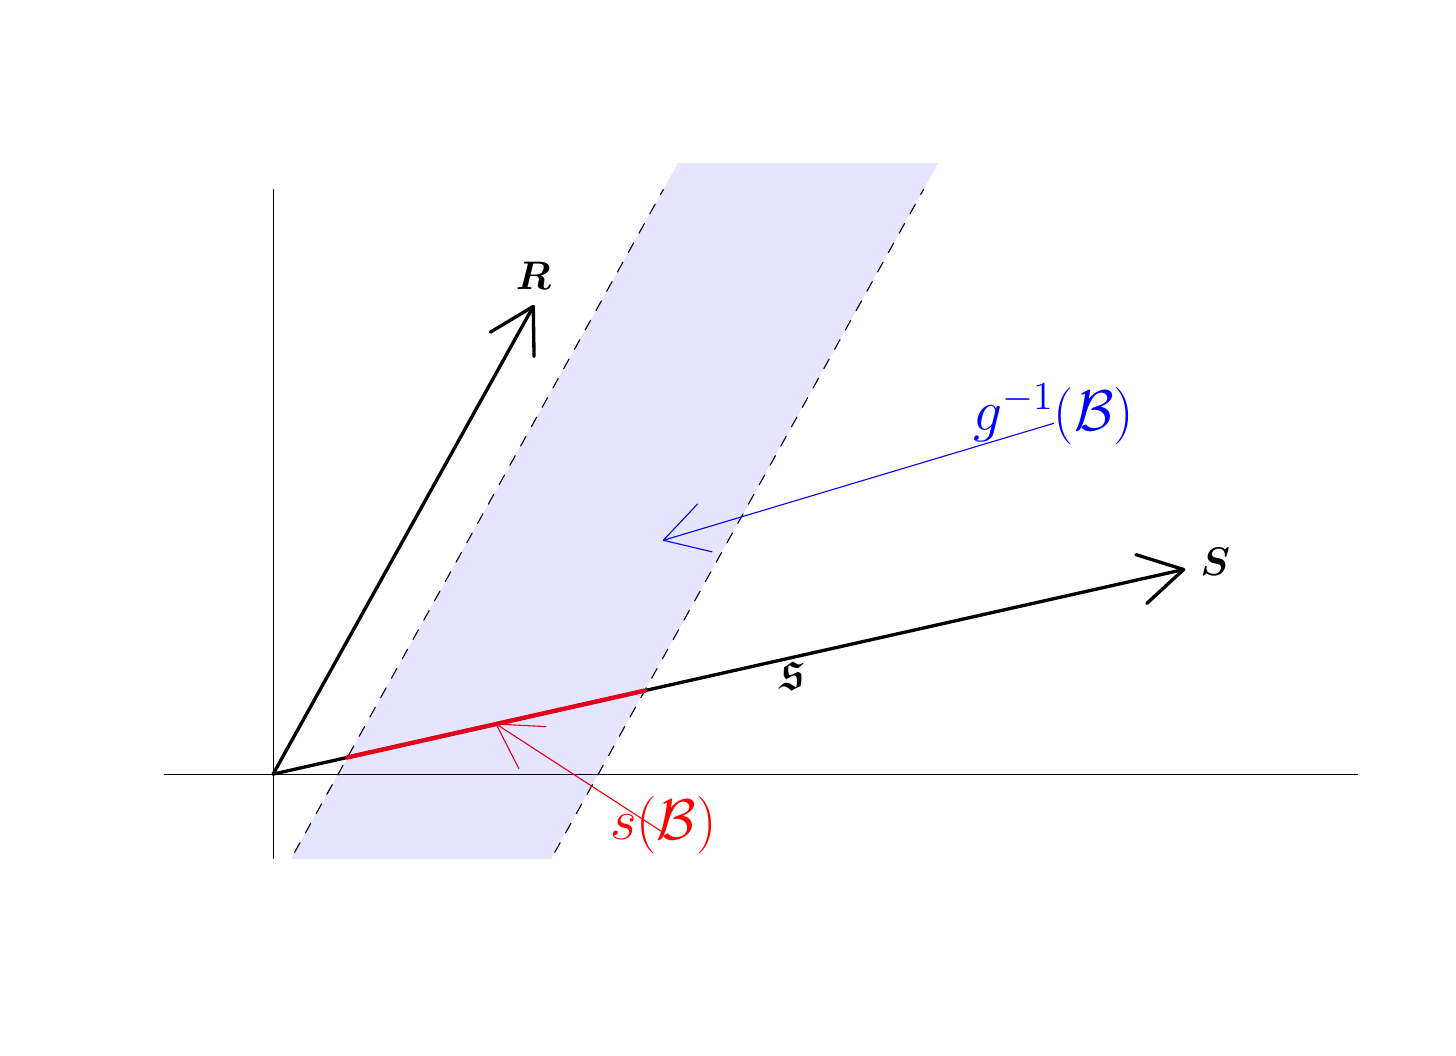
\begin{tikzpicture}[x=1pt,y=1pt]
\definecolor{fillColor}{RGB}{255,255,255}
\path[use as bounding box,fill=fillColor,fill opacity=0.00] (0,0) rectangle (505.89,361.35);
\begin{scope}
\path[clip] ( 49.20, 61.20) rectangle (480.69,312.15);
\definecolor{drawColor}{RGB}{0,0,0}

\path[draw=drawColor,line width= 0.4pt,line join=round,line cap=round] ( 88.68, 49.37) --
	( 88.68,302.86);

\path[draw=drawColor,line width= 0.4pt,line join=round,line cap=round] (  0.00, 91.62) --
	(505.89, 91.62);

\path[draw=drawColor,line width= 1.2pt,line join=round,line cap=round] ( 88.68, 91.62) -- (417.71,165.55);

\path[draw=drawColor,line width= 1.2pt,line join=round,line cap=round] (404.42,153.31) --
	(417.71,165.55) --
	(400.46,170.93);

\node[text=drawColor,anchor=base west,inner sep=0pt, outer sep=0pt, scale=  1.00] at (423.71,163.26) {{\Large ${\bm S}$}};

\node[text=drawColor,anchor=base,inner sep=0pt, outer sep=0pt, scale=  1.00] at (276.70,122.13) {{\huge $\mathfrak{s}$}};

\path[draw=drawColor,line width= 1.2pt,line join=round,line cap=round] ( 88.68, 91.62) -- (182.69,260.61);

\path[draw=drawColor,line width= 1.2pt,line join=round,line cap=round] (182.98,242.54) --
	(182.69,260.61) --
	(167.19,251.33);

\node[text=drawColor,anchor=base,inner sep=0pt, outer sep=0pt, scale=  1.00] at (182.69,266.61) {{\Large ${\bm R}$}};

\path[draw=drawColor,line width= 0.4pt,dash pattern=on 4pt off 4pt ,line join=round,line cap=round] ( 88.68, 49.37) --
	(229.69,302.86);

\path[draw=drawColor,line width= 0.4pt,dash pattern=on 4pt off 4pt ,line join=round,line cap=round] (182.69, 49.37) --
	(323.70,302.86);
\definecolor{drawColor}{RGB}{255,0,0}

\path[draw=drawColor,line width= 1.6pt,line join=round,line cap=round] (115.54, 97.65) --
	(222.98,121.79);
\definecolor{drawColor}{RGB}{0,0,0}

\node[text=drawColor,anchor=base,inner sep=0pt, outer sep=0pt, scale=  1.00] at (229.69, 68.00) {{\huge $\color{red}{s(\mathcal{B})}$}};
\definecolor{drawColor}{RGB}{255,0,0}

\path[draw=drawColor,line width= 0.4pt,line join=round,line cap=round] (229.69, 70.49) -- (169.26,109.72);

\path[draw=drawColor,line width= 0.4pt,line join=round,line cap=round] (187.30,108.78) --
	(169.26,109.72) --
	(177.47, 93.63);
\definecolor{fillColor}{RGB}{0,0,255}

\path[fill=fillColor,fill opacity=0.10] ( 65.18,  7.12) --
	(159.19,  7.12) --
	(347.20,345.10) --
	(253.19,345.10) --
	cycle;
\definecolor{drawColor}{RGB}{0,0,255}

\node[text=drawColor,anchor=base,inner sep=0pt, outer sep=0pt, scale=  1.00] at (370.70,215.86) {{\huge $\color{blue}{g^{-1}(\mathcal{B}})$}};

\path[draw=drawColor,line width= 0.4pt,line join=round,line cap=round] (370.70,218.36) -- (229.69,176.11);

\path[draw=drawColor,line width= 0.4pt,line join=round,line cap=round] (242.09,189.26) --
	(229.69,176.11) --
	(247.27,171.95);
\end{scope}
\end{tikzpicture}

	\caption{Summary of probabilistic forecast reconciliation. The probability that $\bm{y}_{t+h}$ lies in the red line segment under the reconciled probabilistic forecast is defined to be equal to the probability that $\bm{y}_{t+h}$ lies in the shaded blue area under the unreconciled probabilistic forecast. Note that since the smallest hierarchy involves three dimensions, this figure is only a schematic.}\label{fig:probfr_sch}
\end{figure}

Recall that when $s\circ g$ is a projection, the case of point forecast reconciliation can be broken down into three steps.
\begin{compactenum}
\item  $\hat{\bm{y}}_{t+h|t}$ is transformed into coordinates $\tilde{\bm{b}}_{t+h|t}$ and $\tilde{\bm{a}}_{t+h|t}$ via a change of basis.
\item $\tilde{\bm{a}}_{t+h|t}$ is discarded and $\tilde{\bm{b}}_{t+h|t}$ are kept as the bottom-level reconciled forecasts.
\item Reconciled forecasts for the entire hierarchy are recovered via $\tilde{\bm{y}}_{t+h|t}=\bm{S}\tilde{\bm{b}}_{t+h|t}$.
\end{compactenum}
We now outline the analogues to these three steps for probabilistic forecasts when predictive densities are available.

While $\hat{\nu}$ is a probability measure for an $n$-vector $\hat{\bm{y}}_{t+h|t}$, probability statements in terms of a different coordinate system can be made via an appropriate change of basis. Letting $f(.)$ be generic notation for a probability density function, and following the notation from our definition of point forecast reconciliation where $\hat{\bm{y}}_{t+h|t}=\bm{S}\tilde{\bm{b}}_{t+h|t}+\bm{R}\tilde{\bm{a}}_{t+h|t}$, we obtain
\begin{equation}
f(\hat{\bm{y}}_{t+h|t})=f(\bm{S}\tilde{\bm{b}}_{t+h|t}+\bm{R}\tilde{\bm{a}}_{t+h|t})|(\bm{S}~\bm{R})|
\end{equation}
The expression $\hat{\nu}(g^{-1}(\mathcal{B}))$ in Definition~\ref{def:reconprob} is equivalent to the probability statement $\text{Pr}(\hat{\bm{y}}_{t+h|t}\in g^{-1}(\mathcal{B}))$. After the change of basis, this is equivalent to $\text{Pr}(\tilde{\bm{b}}\in \mathcal{B})$, which implies
\begin{align}
\text{Pr}(\hat{\bm{y}}_{t+h|t}\in g^{-1}(\mathcal{B}))&=\int\limits_{g^{-1}(\mathcal{B})}f(\hat{\bm{y}}_{t+h|t})d\hat{\bm{y}}_{t+h|t}\\
&=\int\limits_{\mathcal{B}}\int f(\bm{S}\tilde{\bm{b}}_{t+h|t}+\bm{R}\tilde{\bm{a}}_{t+h|t})|(\bm{S}~\bm{R})|d\tilde{\bm{a}}_{t+h|t}d\tilde{\bm{b}}_{t+h|t}.
\end{align}
After integrating out over $\tilde{\bm{a}}_{t+h|t}$, a step analogous to setting $\tilde{\bm{a}}_{t+h|t}=0$ for point forecasting, we obtain an expression that gives the probability that the reconciled bottom-level series lies in the region $\mathcal{B}$. This corresponds to $\nu(\mathcal{B})$ in Definition~\ref{def:reconprob}. To make a valid probability statement about the entire hierarchy we simply use the bottom-level probabilistic forecasts together with Definition~\ref{def:cohprob}.

%Recall that $\hat{\bm{y}}_{t+h}$ is a set of incoherent point forecasts and the coordinates of $\hat{\bm{y}}_{t+h}$ with respect to the basis $\bm{B}$ are given by \eqref{4.3}. Suppose $\hat{\bm{f}}(\cdot)$ is the probability density of $\hat{\bm{y}}_{t+h}$. Our goal is to reconcile $\hat{\bm{f}}(\cdot)$ such that the density lives on $\mathbb{C}^m$. In order to obtain this reconciled density, we need to project $\hat{\bm{f}}(\hat{\bm{y}}_{t+h})$ onto $\mathbb{C}^m$ along the direction of $\mathbb{N}^{n-m}$.

%Let the density of $\hat{\bm{y}}_{t+h}$ with respect to basis $\bm{B}$ be denoted by $\bm{f_B}(\cdot)$. Then it follows from \eqref{4.3}, and standard results for densities of transformed variables, that
%\begin{equation}\label{4.5}
%\bm{f_B}(\tilde{\bm{b}}_{t+h},\tilde{\bm{t}}_{t+h})=\hat{\bm{f}}(\bm{S}\tilde{\bm{b}}_{t+h}+\bm{R}\tilde{\bm{t}}_{t+h}) \,\Big|\bm{S} ~ \vdots~ \bm{R}\Big|,
%\end{equation}
%where $|\cdot|$ denotes the determinant of a matrix. Now that we have the density of $(\tilde{\bm{b}}'_{t+h} , \tilde{\bm{t}}'_{t+h})'$, the marginal density of $\tilde{\bm{b}}_{t+h}$ can be obtained by integrating \eqref{4.5} over the range of $\tilde{\bm{t}}_{t+h}$. This will result in the reconciled density of the bottom-level series $\tilde{\bm{b}}_{t+h}$,
%\begin{equation}\label{4.6}
%\tilde{\bm{f}}(\tilde{\bm{b}}_{t+h})=\int_{\lim(\tilde{\bm{t}}_{t+h})}\hat{\bm{f}}(\bm{S}\tilde{\bm{b}}_{t+h}+\bm{R}\tilde{\bm{t}}_{t+h})\,  \Big|\bm{S} ~ \vdots~ \bm{R}\Big| \, d\tilde{\bm{t}}_{t+h}.
%\end{equation}
%
%Finally to get the reconciled density of the whole hierarchy, we simply follow Definition~\ref{def:cohprob} to obtain
%\begin{equation}\label{4.7}
%\tilde{\bm{f}}(\tilde{\bm{y}}_{t+h})=\bm{S}\circ \tilde{\bm{f}}(\tilde{\bm{b}}_{t+h}).
%\end{equation}
%This final step will transform every point in the density $\tilde{\bm{f}}(\tilde{\bm{b}}_{t+h})$ to the space $\mathbb{C}^m<\mathbb{R}^n$. The following example illustrates how this method can be used to reconcile an incoherent Gaussian forecast distribution.

\subsubsection*{Example: Gaussian Distributions}

Suppose an unreconciled probabilistic forecast is Gaussian with mean $\hat{\bm{\mu}}$ and variance-covariance matrix $\hat{\bm{\Sigma}}$. The subscripts $t+h|t$ are suppressed for brevity. The unreconciled density
\begin{equation}
  f(\hat{\bm{y}})=(2\pi)^{-n/2}|\hat{\bm{\Sigma}}|^{-1/2}\exp\left\{-\frac{1}{2}\left[(\hat{\bm{y}}-\hat{\bm{\mu}})'\hat{\bm{\Sigma}}^{-1}(\hat{\bm{y}}-\hat{\bm{\mu}})\right]\right\}.
\end{equation}
In an alternative basis,
\begin{equation}
f(\tilde{\bm{b}},\tilde{\bm{a}})=(2\pi)^{-\frac{n}{2}}\Big|\hat{\bm{\Sigma}}\Big|^{-\frac{1}{2}}\Big|(\bm{S} ~  \bm{R})\Big|\exp\{-\frac{1}{2}q\}\,,
\end{equation}
where
\begin{equation}
q=(\bm{S}\tilde{\bm{b}}+\bm{R}\tilde{\bm{a}}-\hat{\bm{\mu}})' \hat{\bm{\Sigma}}^{-1}(\bm{S}\tilde{\bm{b}}+\bm{R}\tilde{\bm{a}}-\hat{\bm{\mu}}).
\end{equation}
The quadratic form $q$ can be rearranged as
\begin{align*}
q& =
\left((\bm{S} ~  \bm{R})\bt-\hat{\bm{\mu}}\right)' \hat{\bm{\Sigma}}^{-1}\left((\bm{S} ~ \bm{R})\bt-\hat{\bm{\mu}}\right),\\
& =
\left(\bt-(\bm{S} ~ \bm{R})^{-1}\hat{\bm{\mu}}_{t+h}\right)' \Big[(\bm{S}  \bm{R})^{-1}\hat{\bm{\Sigma}_{t+h}}\left((\bm{S} ~ \bm{R})^{-1}\right)'\Big]^{-1}
\left(\bt-(\bm{S} ~ \bm{R})^{-1}\hat{\bm{\mu}}_{t+h}\right)\,.
\end{align*}
Recall that
\[
  (\bm{S} ~ \bm{R})^{-1} =
  \begin{pmatrix}(\bm{R}'_\bot \bm{S})^{-1}\bm{R}'_\bot  \\ (\bm{S}'_\bot \bm{R})^{-1}\bm{S}'_\bot \end{pmatrix} :=
  \begin{pmatrix}
  \bm{G} \\\bm{H}
  \end{pmatrix}\,.
\]
Then $q$ can be rearranged further as
\begin{align*}
q& =%\frac{1}{(2\pi)^{\frac{n}{2}}\Big|\hat{\bm{\Sigma}}_{t+h}\Big|^{\frac{1}{2}}\Big|\PQ \Big|}
%\exp \Big\{-\frac{1}{2}
\left[\bt-\PQ\hat{\bm{\mu}}_{t+h}\right]'%\\[-0.5cm]
\left[\PQ\hat{\bm{\Sigma}_{t+h}}\PQ'\right]^{-1}\left[\bt-\PQ\hat{\bm{\mu}}_{t+h}\right] %\Big\},
\\[0.5cm]
 & =%\frac{1}{(2\pi)^{\frac{n}{2}}\Big|\PQ\hat{\bm{\Sigma}_{t+h}}\PQ'\Big|^{\frac{1}{2}}}
%\exp \Big\{-\frac{1}{2}
\begin{pmatrix}\tilde{\bm{b}} - \bm{G}\hat{\bm{\mu}}\\ \tilde{\bm{a}}- \bm{H}\hat{\bm{\mu}}\end{pmatrix}' %&\\[-0.5cm]
%& \hspace*{7cm}
 \left[\PQ\hat{\bm{\Sigma}_{t+h}}\PQ'\right]^{-1}\begin{pmatrix}\tilde{\bm{b}} - \bm{G}\hat{\bm{\mu}}\\ \tilde{\bm{a}}- \bm{H}\hat{\bm{\mu}}\end{pmatrix}. %\Big\}.
\end{align*}
%Since $\Big[\PQ\hat{\bm{\Sigma}_{t+h}}\PQ'\Big] = \begin{pmatrix}
%\bm{P}\hat{\bm{\Sigma}_{t+h}}\bm{P}' & \bm{P}\hat{\bm{\Sigma}_{t+h}}\bm{Q}'
%\bm{Q}\hat{\bm{\Sigma}_{t+h}}\bm{P}' & \bm{Q}\hat{\bm{\Sigma}_{t+h}}\bm{Q}'
%\end{pmatrix}$ we have

Similar manipulations on the determinant of the covariance matrix lead to the following expression for the density:
\begin{align*}
f(\tilde{\bm{b}},\tilde{\bm{a}})&
=(2\pi)^{-\frac{n}{2}}\left|
\begin{pmatrix}
  \bm{G}\hat{\bm{\Sigma}}\bm{G}' & \bm{G}\hat{\bm{\Sigma}}\bm{H}' \\
  \bm{H}\hat{\bm{\Sigma}}\bm{G}' & \bm{H}\hat{\bm{\Sigma}}\bm{H}'
\end{pmatrix}
\right|^{-\frac{1}{2}}
\exp \left\{-\frac{1}{2} \begin{pmatrix}\tilde{\bm{b}} - \bm{G}\hat{\bm{\mu}}\\ \tilde{\bm{a}}- \bm{H}\hat{\bm{\mu}}\end{pmatrix}'\right.\\
&\hspace*{7cm}
\left.\begin{pmatrix}
\bm{G}\hat{\bm{\Sigma}}\bm{G}' & \bm{G}\hat{\bm{\Sigma}}\bm{H}' \\
\bm{H}\hat{\bm{\Sigma}}\bm{G}' & \bm{H}\hat{\bm{\Sigma}}\bm{H}'
\end{pmatrix}^{-1}
\begin{pmatrix}\tilde{\bm{b}} - \bm{G}\hat{\bm{\mu}}\\ \tilde{\bm{a}}- \bm{H}\hat{\bm{\mu}}\end{pmatrix} \right\}.
\end{align*}
Marginalising out $\tilde{\bm{a}}$ leads to the following bottom-level reconciled forecasts:
\begin{equation}\label{ex:2.1}
f(\tilde{\bm{b}})=(2\pi)^{-\frac{m}{2}}\Big|\bm{G}\hat{\bm{\Sigma}}\bm{G}'\Big|^{\frac{1}{2}}
\exp \Big\{-\frac{1}{2} (\tilde{\bm{b}} - \bm{G}\hat{\bm{\mu}})' (\bm{G}\hat{\bm{\Sigma}}\bm{G}')^{-1}(\tilde{\bm{b}} - \bm{G}\hat{\bm{\mu}}) \Big\}.
\end{equation}

%Equation \eqref{ex:2.1} implies $\tilde{\bm{b}}_{t+h} \sim \mathcal{N}(\bm{P}\hat{\bm{\mu}}_{t+h}, \bm{P}\hat{\bm{\Sigma}}_{t+h}\bm{P}')$, where $\bm{P} = (\bm{R}'_\bot \bm{S})^{-1}\bm{R}'_\bot$. Then from \eqref{4.7} it follows that
%\begin{equation}\label{eq:gaussianreconciled}
%\tilde{\bm{f}}(\tilde{\bm{y}}_{t+h})=\tilde{\bm{f}}(\bm{S}\tilde{\bm{b}}_{t+h}).
%\end{equation}
This implies that the reconciled probabilistic forecast for the bottom-level series is $\tilde{\bm{b}}_{t+h} \sim \mathcal{N}(\bm{G}\hat{\bm{\mu}}_{t+h}, \bm{G}\hat{\bm{\Sigma}}_{t+h}\bm{G}')$. The reconciled probabilistic forecasts for the whole hierarchy follow a degenerate Gaussian distribution with mean $\bm{SG}\hat{\bm{\mu}}$ and rank deficient covariance matrix $\bm{SG}\hat{\bm{\Sigma}}_{t+h}\bm{G}'\bm{S}'$.

\subsection{Elliptical distributions}

We now show that the true predictive distribution can be recovered for elliptical distributions by linear reconciliation via pre-multiplication and translation respectively by a matrix we denote ${\bm G}_{opt}$ and vector we denote  ${\bm d}_{opt}$. Here, for any square matrix $\bm{C}$, $\bm{C}^{1/2}$ and $\bm{C}^{-1/2}$ are defined to satisfy $\bm{C}^{1/2}(\bm{C}^{1/2})'=\bm{C}$ and $\bm{C}^{-1/2}(\bm{C}^{-1/2})'=\bm{C}^{-1}$, for example $\bm{C}^{1/2}$ may be obtained via the Cholesky or eigenvalue decompositions.

\begin{theo}[Reconciliation for Elliptical Distributions]
	Let an unreconciled probabilistic forecast come from the elliptical class with location parameter $\hat{\bm{\mu}}$ and scale matrix $\hat{\bm{\Sigma}}$. Let the true predictive distribution of $\bm{y}_{t+h|t}$ also belong to the elliptical class with location parameter $\bm{\mu}$ and scale matrix $\bm{\Sigma}$. Then the linear reconciliation mapping $g(\breve{\bm{y}})=\bm{G}_{opt}\breve{\bm{y}}+\bm{d}_{opt}$ with $\bm{G}_{opt}={\bm{a}}{\bm\Sigma}^{-1/2}$ and $\bm{d}_{opt}=\bm{\mu}-\bm{S}\bm{G}_{opt}\hat{\bm{\mu}}$ recovers the true predictive density where ${\bm{a}}$ is any $m\times n$ matrix such that ${\bm{a}}{\bm{a}}'=\bm{\Omega}$ and $\bm{\Omega}$ is a sub-matrix of $\bm{\Sigma}$ corresponding to the bottom-level series.
\end{theo}

\begin{proof}
   Since elliptical distributions are closed under affine transformations, and are closed under marginalisation, reconciliation of an elliptical distribution yields an elliptical distribution (although the unreconciled and reconciled distributions may be different members of the class of elliptical distributions). The scale matrix of the reconciled forecast is given by $\bm{S}\bm{G}_{opt}\bm{\Sigma}\bm{G}_{opt}'\bm{S}'$, while the location matrix is given by $\bm{S}\bm{G}_{opt}\hat{\bm{\mu}}+\bm{d}_{opt}$. The reconciled scale matrix is
   \[
     \tilde{\bm{\Sigma}}_{opt}
       = \bm{S}{\bm{a}}{\bm\Sigma}^{-1/2}\bm{\Sigma}\left({\bm\Sigma}^{-1/2}\right)'{\bm{a}}'\bm{S}'
       = \bm{S}\bm{\Omega}\bm{S}'
       = \bm{\Sigma}.
   \]
   For the choices of $\bm{G}_{opt}$ and $\bm{d}_{opt}$ given above, the reconciled location vector is
   \[
     \tilde{\bm{\mu}}_{opt}= \bm{S}\bm{G}_{opt}\hat{\bm{\mu}}+\bm{\mu}-\bm{S}\bm{G}_{opt}\hat{\bm{\mu}}
   = \bm{\mu}.
   \]
\end{proof}

A number of insights can be drawn from this theorem. First, although a linear function $g(.)$ can be used to recover the true predictive in the elliptical case, the same does not hold in general. Second, $g(.)$ is not, in general, a projection matrix. The conditions for which a the true predictive density can be recovered by a projection are given below.

\begin{theo}[True predictive via projection]
	Assume that the true predictive distribution is elliptical with location $\bm{\mu}$ and scale $\bm{\Sigma}$. Consider reconciliation via a projection $g(\bm{y})=(\bm{R}'_{\perp}\bm{S})^{-1}\bm{R}'_{\perp}\bm{y}$. The true predictive distribution can be recovered via reconciliation of an elliptical distribution with location $\hat{\bm{\mu}}$ and scale $\hat{\bm{\Sigma}}$  when the following conditions hold:
	\begin{align}
	sp(\hat{\bm\mu}-\bm{\mu})&\subset sp(\bm{R})\\
    sp(\hat{\bm{\Sigma}}^{1/2}-\bm{\Sigma}^{1/2})&\subset sp(\bm{R})\\
	\end{align}
\end{theo}

\begin{proof}
	The reconciled location vector will be given by
	\begin{align*}
		\tilde{\bm{\mu}}&=\bm{S}(\bm{R}'_{\perp}\bm{S})^{-1}\bm{R}'_{\perp}\hat{\bm{\mu}}\\
		&=\bm{S}(\bm{R}'_{\perp}\bm{S})^{-1}\bm{R}'_{\perp}\left(\hat{\bm{\mu}}+\bm{\mu}-\bm{\mu}\right)\\
		&=\bm{S}(\bm{R}'_{\perp}\bm{S})^{-1}\bm{R}'_{\perp}\bm{\mu}+\bm{S}(\bm{R}'_{\perp}\bm{S})^{-1}\bm{R}'_{\perp}\left(\hat{\bm{\mu}}-\bm{\mu}\right).
	\end{align*}
  Since $\bm{S}(\bm{R}'_{\perp}\bm{S})^{-1}\bm{R}'_{\perp}$ is a projection onto $\mathfrak{s}$ and $\bm{\mu}\in\mathfrak{s}$, the first term simplifies to $\bm{\mu}$. If $\bm{\mu}-\hat{\bm{\mu}}$ lies in the span of $\bm{R}$, then multiplication by $\bm{R}'_{\perp}$ reduces the second term to $\bm{0}$. By a similar argument it can be shown that $\tilde{\bm{\Sigma}}^{1/2}=\bm{\Sigma}^{1/2}$. The closure property of elliptical distributions under affine transformations ensures that the full true predictive distribution can be recovered.
\end{proof}

Although these conditions will rarely hold in practice and only apply to a limited class of distributions, they do provide some insight into selecting a projection for reconciliation. If the value of $\hat{\bm{\mu}}$ were equi-probable in all directions, then a projection orthogonal to $\mathfrak{s}$ would be a sensible choice for $\bm{R}$ since it would in some sense represent a `median' direction for $\bm{\mu}-\hat{\bm{\mu}}$. However, the one-step-ahead in-sample errors are usually correlated suggesting that $\hat{\bm{\mu}}$ is more likely to fall in some directions than others. Therefore an orthogonal projection after transformation by the inverse of the one-step-ahead in-sample error covariance matrix may be more intuitively appealing. This is exactly what the MinT projection provides, and as simulations will show in Section~\ref{sec:gaussian}, this projection leads to the best empirical results.

%However, these expressions do provide some insight on why some choices for $\bm{G}$ in the point forecast reconciliation literature may also work well for probabilistic forecasts. To illustrate, first rearrange the equation for the optimal value of  $\bm{G}_{opt}={\bm\Omega}^{1/2}\hat{\bm\Sigma}^{-1/2}$ as ${\bm\Omega}^{1/2}=\bm{G}_{opt}\hat{\bm\Sigma}^{1/2}$. For arbitrary $\bm{G}\hat{\bm\Sigma}^{1/2}$ is an approximation for ${\bm\Omega}^{1/2}$. This approximation has similarities with the way bottom-level estimates are produced for point forecast reconciliation. Rather than mapping a vector of point forecasts to reconcilied bottom-level forecasts, the columns of  $\hat{\bm\Sigma}^{1/2}$ are mapped to an approximation of the columns of ${\bm\Omega}^{1/2}$. The value for $\tilde{\bm{\mu}}_{opt}$ includes a projection of $\hat{\bm{\mu}}$ onto $\mathfrak{s}$. While it is infeasible to obtain the translation $\bm{d}$, it is worthwhile noting that this measures the difference between the reconciled mean and true mean.

\section{Evaluation of hierarchical probabilistic forecasts}\label{sec:evaluation}

The necessary final step in hierarchical forecasting is to make sure that our forecast distributions are accurate. In general, forecasters prefer to maximize the sharpness of the forecast distribution subject to calibration \citep{Gneiting2014}. Therefore the probabilistic forecasts should be evaluated with respect to these two properties.

Calibration refers to the statistical compatibility between probabilistic forecasts and realizations. In other words, random draws from a perfectly calibrated forecast distribution should be equivalent in distribution to the realizations. On the other hand, sharpness refers to the spread or the concentration of the predictive distributions and it is a property of the forecasts only. The more concentrated the forecast distributions, the sharper the forecasts \citep{Gneiting2008}. However, independently assessing the calibration and sharpness will not help to properly evaluate the probabilistic forecasts. Therefore we need to assess these properties simultaneously using scoring rules.

Scoring rules are summary measures obtained based on the relationship between the forecast distributions and the realizations. In some studies, researchers take the scoring rules to be positively oriented, in which case the scores should be maximized \citep{Gneiting2007}. However, scoring rules have also been defined to be negatively oriented, and then the scores should be minimized \citep{Gneiting2014}. We follow the latter convention here.

Let $P$ be a forecast distribution and let $Q$ be the true data generating process respectively. Furthermore let $\omega$ be a realization from $Q$. Then a scoring rule is a function $S(P,\omega)$ that maps $P,\omega$ to $\mathbb{R}$. It is a ``proper'' scoring rule if
\begin{equation}\label{eq:(3.1.)}
\E_{\bm{Q}}[S(Q,\omega)] \le \E_{\bm{Q}}[S(P,\omega)] ,
\end{equation}
where $\E_{Q}[S(P,\omega)]$ is the expected score under the true distribution $Q$ \citep{Gneiting2008, Gneiting2014}. When this inequality is strict, the scoring rule is said to be strictly proper.

In the context of probabilistic forecast reconciliation there could be two motivations for using scoring rules. The first is to compare unreconciled densities to reconciled densities. Reconciliation itself is a valuable goal since it can be important in aligning decision making across, for example, different units of an enterprise. In the point forecasting literature, forecast reconciliation has also been shown to improve forecast performance \citep{AthEtAl2017, Wickramasuriya2017}. It will be worthwhile to see whether the same holds in the probabilistic forecasting case. The second motivation for using scoring rules is to compare two or more sets of reconciled probabilistic forecasts to one another. The objective here is to evaluate which reconciliation mapping $g(.)$ works best in practice.

\subsection{Univariate scoring rules}

One way to evaluate hierarchical probabilistic forecasts is via the application of univariate scoring rules to each variable in the hierarchy. A summary can be taken of the expected scores across each margin, for example a mean or median. In the simulations of Section~\ref{sec:gaussian}, we consider two scoring rules. The log score is given by the log density, in this case for each margin of the probabilistic forecast. The cumulative rank probability score generalises mean square error and is given by
\begin{align} \label{eq:CRPS}
\text{CRPS}(\breve{F}_i,y_{i}) &=\int \left(\breve{F}_i(\breve{Y}_i)-\mathbb{1}(y_i<y_{i})\right)d\breve{Y}_i\\ &=\E_{\breve{Y}_i}|\breve{Y}_{i}-y_{i}| - \frac{1}{2}\E_{\breve{Y}_i}|\breve{Y}_{i}-\breve{Y}^*_{i}|\,,
\end{align}
where $\breve{F}_i$ is the cumulative distribution function of the $i$th margin of the probabilistic forecast, $\breve{Y}_i$ and $\breve{Y}^*_{i}$ are independent copies of a random variable with distribution $\breve{F}_i$, and $y_i$ is the outcome of the $i$th margin. The expectations in the second line can be approximated by Monte Carlo when a sample from the predictive distribution is available.

An advantage to this approach is that it allows the forecaster to evaluate the levels and individual series of the hierarchy where the gains from reconciliation are greatest. For this reason this approach has been used in the limited literature on probabilistic forecasting for hierarchies \citep{BenTaieb2017, JeoEtAl2018} to date. A major shortcoming of this approach however, is that evaluating univariate scores on the margins does not account for the dependence in the hierarchy.

\subsection{Multivariate scoring rules}

While a number of alternative proper scoring rules are available for univariate forecasts, the multivariate case is somewhat more limited. Here we focus on three scoring rules: the log score, the energy score and the variogram score. %These are summarized in table~\ref{table:scoringrules}.
%
%\begin{table}[!bh]
%  \caption{Scoring rules to evaluate multivariate forecast densities. Here, $\breve{\bm{y}}_{T+h}$ and $\breve{\bm{y}}^*_{T+h}$ are two independent random vectors from the coherent forecast distribution $\breve{\bm{F}}$ with density function $\breve{\bm{f}}(\cdot)$ at time $T+h$, and $\bm{y}_{T+h}$ is the vector of realizations. Further, $\breve{Y}_{T+h,i}$ and $\breve{Y}_{T+h,j}$ are the $i$th and $j$th components of the vector $\breve{\bm{Y}}_{T+h}$. The variogram score is given for order $p$, where $w_{ij}$ denote non-negative weights.}\label{table:scoringrules}
%  \centering\small\setstretch{1.3}
%  \begin{tabular}{@{}lp{8.1cm}l@{}}
%    \toprule
%    \textbf{Scoring rule}  & \textbf{Expression} & \textbf{Reference}           \\
%    \midrule
%    \text{Log score}       &
%    $\text{LS}(\breve{\bm{F}},\bm{y}_{T+h}) = -\log {\breve{\bm{f}}(\bm{y}_{T+h})}$ &
%    \citet{Gneiting2007}  \\\\[-0.2cm]
%    \text{Energy score}    &
%    $\text{ES}(\breve{\bm{Y}}_{T+h},\bm{y}_{T+h}) =
%    \E_{\breve{\bm{F}}}
%    \|\breve{\bm{Y}}_{T+h}-\bm{y}_{T+h}\|^\alpha -$ \par\hfill
%    $\frac{1}{2}\E_{\breve{\bm{F}}}\|\breve{\bm{Y}}_{T+h}-\breve{\bm{Y}}^*_{T+h}\|^\alpha$, \,\, $\alpha \in (0,2]$ &
%    \citet{Gneiting2008}  \\\\[-0.2cm]
%    \text{Variogram score} &
%    $\text{VS}(\breve{\bm{F}}, \bm{y}_{T+h}) =
%    \sum\limits_{i=1}^{n}
%    \sum\limits_{j=1}^{n}
%    w_{ij}\Big(|y_{T+h,i} - y_{T+h,j}|^p -$ \par\hfill
%    $\E_{\breve{\bm{F}}}|\breve{Y}_{T+h,i}-\breve{Y}_{T+h,j}|^p\Big)^2$     &
%    \citet{SCHEUERER2015} \\
%    \bottomrule
%  \end{tabular}
%\end{table}

The log score can be approximated using a sample of values from the probabilistic forecast density \citep{Jordan2017}; however it is more commonly used when a parametric form for the density is available for the probabilistic forecast.

The energy score on the other hand can be defined in terms of the characteristic function of the probabilistic forecast, but the representation in terms of expectations leads itself to easy computation when samples from the probabilistic forecast are available. An interesting limiting case is where $\alpha=2$, where it can be easily shown that energy score simplifies to mean squared error around the mean of the predictive distribution. In this limiting case, the energy score is proper but not strictly proper. \citet{Pinson2013a} also argue that the energy score has low discriminative ability for incorrectly specified covariances, even though it discriminates the misspecified means well.

In contrast, \citet{SCHEUERER2015} have shown that the variogram score has a higher discrimination ability for misspecified means, variances and correlation structures than the energy score. When $\breve{\bm{y}}$ is a random variable from probabilistic forecast $\breve{F}$, the empirical variogram score is defined as
\begin{equation}
\text{VS}(\breve{F}, \bm{y}) = \displaystyle\sum_{i=1}^{n}\displaystyle\sum_{j=1}^{n}w_{ij}\left(|y_{i} - y_{j}|^p - E_{\breve{Y}_i,\breve{Y}_j} |\breve{Y}_{i}-\breve{Y}_{j}|^p\right)^2.
\end{equation}
\citet{SCHEUERER2015} recommend using $p=0.5$.

%For example, assume you have a Gaussian coherent predictive density $\bm{\tilde{f}}_{T+h}$. Then the log score is given by

%\begin{equation}
%LS(\bm{\tilde{f}_{T+h},y_{T+h}}) = -\log \left(\frac{1}{(2\pi)^{\frac{m}{2}}|\bm{\tilde{\Sigma}}_{T+h}|^{\frac{1}{2}}}\exp\left[-\frac{1}{2}(\bm{y}_{T+h}-\bm{\tilde{\mu}}_{T+h})^T %\bm{\tilde{\Sigma}_{T+h}}^{-1}(\bm{y}_{T+h}-\bm{\tilde{\mu}}_{T+h})\right]\right),
%\end{equation}

%
%where $\bm{\tilde{\mu}}_{T+h}$ and $\bm{\tilde{\Sigma}}_{T+h}$ are the coherent mean and variance-covariance matrix of the predictive Gaussian density and both lies in the linear %subspace spanned by $\mathbb{C}^m$. Then $\bm{\tilde{\Sigma}}_{T+h}$ is always a singular matrix and hence the determinant will be zero. Therefore the density function of %degenerate Gaussian distribution is undefined. However, we could use the pseudo determinant, i.e. product of positive eigenvalues and the pseudo inverse to calculate the log score %to compare the predictive ability of coherent forecast densities.

\subsubsection{Comparing unreconciled forecasts to reconciled forecasts}

For both reconciled and unreconciled densities it is possible to obtain a density from the probability measures defined in Section~\ref{sec:definitions}. Therefore it may seem sensible to compare unreconciled densities to reconciled densities on the basis of log score. However, the following theorem shows that using the log score may fail in the case of multivariate distributions with a degeneracy.

\begin{theo}[Impropriety of log score]
	When the true data generating process is coherent, then the log score is improper with respect to the class of incoherent measures.
\end{theo}

\begin{proof}
Consider a rotated version of hierarchical time series, $\bm{z}_t=\bm{U}\bm{y}_t$, so that the first $m$ elements of $\bm{z}_t$ denoted $\bm{z}^{(1)}_t$ are unconstrained, while the remaining $n-m$ elements denoted $\bm{z}^{(2)}_t$ equal $0$ when the aggregation constraints hold. An example of the $n\times n$ $\bm{U}$ is the matrix of left singular vectors of $\bm{S}$. %For a non-degenerate probability measure on $\mathbb{R}^n$, the density is the Radon-Nikodym derivative with respect to the usual Lesbegue measure on $\mathbb{R}^n$. %For a coherent probability measure the density after rotation is the Radon-Nikodym derivative with respect to the usual Lesbegue measure on $\mathbb{R}^m$.

Consider the case where the true predictive density is $f_1(\bm{z}^{(1)}_t)\mathbb{1}\left(\bm{z}^{(2)}_t=\bm{0}\right)$, and we evaluate an incoherent density given by $f_1(\bm{z}^{(1)}_t)f_2(\bm{z}^{(2)}_t)$, where $f_2$ is highly concentrated around $0$ but still non-degenerate. For example, $f_2$ may be Gaussian with variance $\sigma^2{\bm{I}}$ with $\sigma^2 < (2\pi)^{-1}$. The log score under the true data generating process is
\[
S\left(f,\bm{z}^{(1)}_t\right) = -\log f_1\left(\bm{z}^{(1)}_t\right),
\]
while that of the unreconciled density is
\begin{align}
S\left(\hat{f},\bm{z}^{(1)}_t\right) &= -\log f_1(\bm{z}^{(1)}_t)-f_2(\bm{z}^{(1)}_t)\\
&= -\log f_1(\bm{z}^{(1)}_t)+\frac{n-m}{2}\log(2\pi\sigma^2)\\
&<-\log f_1(\bm{z}^{(1)}_t)=S\left(f,\bm{z}^{(1)}_t\right).
\end{align}
After taking expectations $ES(f,f) > ES(\hat{f},f)$, violating the condition in Equation~\eqref{eq:(3.1.)} for a proper scoring rule.
\end{proof}

A similar issue also arises when discrete random variables are modelled as if they were continuous, an issue discussed in Section~4.1 of \citet{Gneiting2007}. This implies that the log score should be avoided when comparing reconciled and unreconciled probabilistic forecasts.

\subsubsection{Comparing reconciled forecasts to one another}

Coherent probabilistic forecasts can be completely characterised in terms of basis series; if a probabilistic forecast is available for the basis series, then a probabilistic forecast can be recovered for the entire hierarchy via Definition~\ref{def:cohprob}. This may suggest that it is adequate to merely compare two coherent forecasts to one another using the basis series only. We now show how this depends on the specific scoring rule used.

For the log score, suppose the coherent probabilistic forecast has density $f(\bm{b})$. The density for the full hierarchy is given by $f(\bm{y})=f(\bm{Sb})=f(\bm{b})J^{-1}$, where $J=\prod_{j=1}^{m}\lambda_j$ is a pseudo-determinant of the non-square matrix $\bm{S}$ and $\lambda_j$ are the non-zero singular values of $\bm{S}$. Therefore for any coherent density, the log score of the full hierarchy differs from the log score for the bottom-level series by the term $log(J)$. This term depends only on the structure of the hierarchy and is fixed across different reconciliation methods. Therefore if one method achieves a lower expected log score compared to an alternative method using the bottom-level series only, the same ordering is preserved when an assessment is made on the basis of the full hierarchy.

The same property does not hold for all scores in general. For example, the energy score can be expressed in terms of expectations of norms. In general, since norms are invariant under orthogonal rotations, the energy score is also invariant under orthogonal transformations \citep{Szekely2013,Gneiting2007}. In the context of two coherent forecasts, the same is true of a semi-orthogonal transformation from a lower dimensional basis series to the full hierarchy. However, when $\bm{S}$ is the usual summing matrix, it is not semi-orthogonal. Therefore the energy score computed on the bottom-level series will differ from the energy score computed using the full hierarchy and the ordering of different reconciliation methods may change depending on the basis series used. In this case we recommend computing the energy score using the full hierarchy. Although the discussion here is related to energy score, the same logic holds for other multivariate scores, for example the variogram score.

The properties of multivariate scoring rules in the context of evaluating reconciled probabilistic forecasts are summarised in Table~\ref{tab:prop}.

\begin{table}
	\centering
	\begin{tabular}{rll}
	& Coherent v Incoherent &Coherent v Coherent\\
	\hline
	Log Score & Not proper & Ordering preserved if compared using\\ &&bottom-level only\\
	Energy/ & Proper & Full hierarchy should be used\\
	Variogram Score & &\\
	\hline
    \end{tabular}
	\caption{Summary of properties of scoring rules in the context of reconciled probabilistic forecasts.}
	\label{tab:prop}
\end{table}

%\subsection{Comparison of coherent and incoherent forecast densities}
%
%It is also important to assess how the coherent or reconciled forecast densities improve the predictive ability compared to the incoherent forecasts. Clearly, we cannot use multivariate scoring rules, even for the basis set of series, since the coherent and incoherent forecast densities lie in two different metric spaces.
%
%However we could compare the individual margins of the forecast density of the hierarchy using univariate proper scoring rules. The widely used Continuous Ranked Probability Score (CRPS) could then be used. This is defined as
%%\begin{equation} \label{eq:(3.6)}
%%\text{CRPS}(\breve{F}_i,y_{T+h,i}) = \E_{\breve{F}_i}|\breve{Y}_{T+h,i}-y_{T+h,i}| - \frac{1}{2}\E_{\breve{F}_i}|\breve{Y}_{T+h,i}-\breve{Y}^*_{T+h,i}|,
%%\end{equation}
%where $\breve{Y}_{T+h,i}$ and $\breve{Y}^*_{T+h,i}$ are two independent copies from the $i$th reconciled marginal forecast distribution $\tilde{F}_i$ of the hierarchy, and $y_{T+h,i}$ is the $i$th realization from the true marginal distribution $G_i$. We could also use univariate log scores, for which we could assume a parametric forecast distribution.

\section{Simulation study}\label{sec:gaussian}

%An important special case for probabilistic forecasting arises when we can assume a multivariate Gaussian distribution. That is, suppose all the historical data in the hierarchy follows a multivariate Gaussian distribution, $\bm{y}_T \sim \mathcal{N}(\bm{\mu}_T, \bm{\Sigma}_T)$, where both $\bm{\mu}_T$ and $\bm{\Sigma}_T$ live in $\mathbb{C}^m$ by nature of the hierarchical structure of the data. We are interested in estimating the predictive Gaussian distribution of $\bm{Y}_{T+h}| \bm{\mathcal{I}}_T$, where $\bm{\mathcal{I}}_T= \{\bm{y}_1,\bm{y}_2,\dots.,\bm{y}_T\}$, which should also live in $\mathbb{C}^m$.
%
%It is well known that the optimal point forecasts with respect to the minimal mean square error are given by the conditional expectations, $\E[Y_{T+h,i}\mid y_{1,i},\dots,y_{T,i}],$ $i=1,\dots,n$. Suppose we independently fit time series models for each series in the hierarchy. Then the point forecasts, $\hat{Y}_{T+h,i}$, from the estimated models are unbiased and consistent estimators of $\E[Y_{T+h,i}\mid y_{1,i},\dots,y_{T,i}]$, assuming the parameter estimates of the fitted models are unbiased and asymptotically consistent. \todo{Only for linear models?}
%
%For example, suppose the data from $i$th series follows a ARMA$(p,q)$ model. i.e.,
%\[
%Y_{t,i}=\alpha_1Y_{t-1,i}+\dots+\alpha_pY_{t-p,i}+\varepsilon_t + \beta_1\varepsilon_{t-1,i}+\dots+\beta_q\varepsilon_{t-q,i},
%\]
%where $\varepsilon_t \sim \mathcal{NID}(0, \sigma_i^2)$. Then,
%\[
%\E[Y_{T+h,i}\mid y_{1,i},\dots,y_{T,i}] = \alpha_1Y_{T+h-1,i}+\dots+\alpha_pY_{T+h-p,i}+ \beta_1\varepsilon_{T+h-1,i}+\dots+\beta_q\varepsilon_{T+h-q,i}.
%\]
%
%Since $\bm{\alpha} = (\alpha_1,\dots,\alpha_p)'$ and $\bm{\beta} = (\beta_1,\dots,\beta_q)'$ are unknown in practice and thus estimated using the maximum likelihood method. Let $\hat{\bm{\alpha}}$ and $\hat{\bm{\beta}}$ denote the maximum likelihood estimates of $\bm{\alpha}$ and $\bm{\beta}$ respectively. \citet{Yao2006} showed that $\hat{\bm{\alpha}}$ and $\hat{\bm{\beta}}$ are asymptotically consistent estimators. Thus the point forecasts from this estimated model, $\hat{Y}_{T+h,i}$, will also be a consistent estimator for $\E[Y_{T+h,i}\mid y_{1,i},\dots,y_{T,i}]$. i.e.,
%\begin{equation} \label{eq:(6.01)}
%\hat{Y}_{T+h,i} \overset{p}{\to} \E[Y_{T+h,i}\mid y_{1,i},\dots,y_{T,i}] \quad \text{as} \quad T \to \infty.
%\end{equation}
%
%Let $\hat{\bm{Y}}_{T+h}=(\hat{Y}_{T+h,1},\dots,\hat{Y}_{T+h,n})'$ and suppose \eqref{eq:(6.01)} holds for $i=1,\dots,n$. Then from Slutsky's theorem it follows that
%\begin{equation}\label{eq:(6.02)}
%\hat{\bm{Y}}_{T+h} \overset{p}{\to} \E[\bm{Y}_{T+h}|\bm{\mathcal{I}}_T] \quad \text{as} \quad T \to \infty.
%\end{equation}
%Further, let the forecast error due to $\hat{\bm{Y}}_{T+h}$ be given by
%\begin{equation}
%\hat{\bm{e}}_{T+h} = \bm{Y}_{T+h}-\hat{\bm{Y}}_{T+h},
%\end{equation}
%and consider the variance of $\hat{\bm{e}}_{T+h}$,
%\begin{align*}
%\E[(\bm{Y}_{T+h} - \hat{\bm{Y}}_{T+h})(\bm{Y}_{T+h} - \hat{\bm{Y}}_{T+h})'|\bm{\mathcal{I}}_T] = &
%\E[(\bm{Y}_{T+h} - \E(\bm{Y}_{T+h}|\bm{\mathcal{I}}_T) + \E(\bm{Y}_{T+h}|\bm{\mathcal{I}}_T)- \hat{\bm{Y}}_{T+h})\\
%& \quad
%(\bm{Y}_{T+h} - \E(\bm{Y}_{T+h}|\bm{\mathcal{I}}_T) + \E(\bm{Y}_{T+h}|\bm{\mathcal{I}}_T) - \hat{\bm{Y}}_{T+h})'|\bm{\mathcal{I}}_T],\\
%= &
%\E[(\bm{Y}_{T+h} - \E(\bm{Y}_{T+h}|\bm{\mathcal{I}}_T))(\bm{Y}_{T+h} - \E(\bm{Y}_{T+h}|\bm{\mathcal{I}}_T))'|\bm{\mathcal{I}}_T]\\
%& \quad
%+ \E[\E(\bm{Y}_{T+h}|\bm{\mathcal{I}}_T) - \hat{\bm{Y}}_{T+h})(\E(\bm{Y}_{T+h}|\bm{\mathcal{I}}_T) - \hat{\bm{Y}}_{T+h})'|\bm{\mathcal{I}}_T]\\
%& \quad
%+  \E[(\bm{Y}_{T+h} - \E(\bm{Y}_{T+h}|\bm{\mathcal{I}}_T))(\E(\bm{Y}_{T+h}|\bm{\mathcal{I}}_T) - \hat{\bm{Y}}_{T+h})'|\bm{\mathcal{I}}_T]\\
%&  \quad
%+ \E[\E(\bm{Y}_{T+h}|\bm{\mathcal{I}}_T) - \hat{\bm{Y}}_{T+h})(\bm{Y}_{T+h} - \E(\bm{Y}_{T+h}|\bm{\mathcal{I}}_T))'|\bm{\mathcal{I}}_T].
%\end{align*}
%
%From \eqref{eq:(6.02)} it immediately follows that
%\begin{align*}
%&\E[(\bm{Y}_{T+h} - \hat{\bm{Y}}_{T+h})(\bm{Y}_{T+h} - \hat{\bm{Y}}_{T+h})'|\bm{\mathcal{I}}_T] \overset{p}{\to} \E[(\bm{Y}_{T+h} - \E(\bm{Y}_{T+h}|\bm{\mathcal{I}}_T))(\bm{Y}_{T+h} - \E(\bm{Y}_{T+h}|\bm{\mathcal{I}}_T))'|\bm{\mathcal{I}}_T].
%\end{align*}
%That is,
%\begin{equation}
%\bm{W}_{T+h} \overset{p}{\to} \text{Var}(\bm{Y}_{T+h}|\bm{\mathcal{I}}_T) \quad \text{as} \quad T \to \infty,
%\end{equation}
%where $\E[(\bm{Y}_{T+h} - \hat{\bm{Y}}_{T+h})(\bm{Y}_{T+h} - \hat{\bm{Y}}_{T+h})'|\bm{\mathcal{I}}_T] = \bm{W}_{T+h}$.
%
%Even though $\hat{\bm{Y}}_{T+h}$ and $\bm{W}_{T+h}$ are asymptotically consistent estimators for $\E(\bm{Y}_{T+h}|\bm{\mathcal{I}}_T)$ and $\text{Var}(\bm{Y}_{T+h}|\bm{\mathcal{I}}_T)$ respectively, they are not coherent since they do not lie in the coherent subspace. Thus the Gaussian forecast distribution with mean $\hat{\bm{Y}}_{T+h}$ and variance $\bm{W}_{T+h}$ will be incoherent, and we denote it by
%\begin{equation}\label{eq:(6.03)}
%\widehat{\bm{Y}_{T+h,i}|\bm{\mathcal{I}}_T} \sim \mathcal{N}(\hat{\bm{Y}}_{T+h}, \bm{W}_{T+h})
%\end{equation}
%
%Since our primary objective is to find the coherent forecast density of the hierarchy, we need to reconcile \eqref{eq:(6.03)}. Using \eqref{eq:gaussianreconciled}, the reconciled Gaussian forecast distribution is then given by
%\begin{equation}\label{eq:(6.04)}
%\widetilde{\bm{Y}_{T+h,i}|\bm{\mathcal{I}}_T} \sim \mathcal{N}(\bm{SP}\hat{\bm{Y}}_{T+h}, \bm{SP}\bm{W}_{T+h}\bm{P}'\bm{S}'),
%\end{equation}
%where $\bm{P} = (\bm{R}'_\bot \bm{S})^{-1}\bm{R}'_\bot$.
%
%\textbf{Result 1}: Choosing $\bm{R}'_\bot = \bm{S}'\bm{W}_{T+h}^{-1}$ will ensure that at least the mean of the predictive Gaussian distribution is optimally reconciled with respect to the energy score.
%
%Result 1 can be easily shown as follows. From \eqref{eq:(5.1)}, the energy score at the upper limit of $\alpha=2$ is given by $\|\bm{y}_{T+h}-\bm{SP}\hat{\bm{y}}_{T+h}\|^2$. Then the expectation of the energy score with respect to the true distribution is equivalent to the trace of mean squared forecast error; i.e.,
%\[
%\E_{\bm{G}}[eS(\bm{\tilde{Y}_{T+h},y_{T+h}})]= \text{Tr}\{\E_{\bm{y}_{T+h}}[(\bm{Y}_{T+h}-\bm{SP}\hat{\bm{Y}}_{T+h})(\bm{Y}_{T+h}-\bm{SP}\hat{\bm{Y}}_{T+h})'|\mathcal{I}_{T}]\}.
%\]
%
%From Theorem 1 of \citet{Wickramasuriya2017} it immediately follows that $\bm{P} = (\bm{S}'\bm{W}_{T+h}^{-1}\bm{S})^{-1}\bm{S}'\bm{W}_{T+h}^{-1}$ minimizes the expected energy score, if we constrain the reconciled forecasts to be unbiased. Thus we have $\bm{R}'_\bot = \bm{S}'\bm{W}_{T+h}^{-1}$.
%
%It should be noted that $\bm{W}_{T+h}$ can be estimated in different ways, which yields different estimates of $\bm{R}'_\bot$. Table~\ref{table:2} summarizes some of these methods.
%

%All of these forecasting methods are well-established in the context of point forecast reconciliation \citep{Hyndman2011, Hyndman2016,Wickramasuriya2017}. Here, we are showing how these reconciliation methods can be used in the context of probabilistic forecast reconciliation, at least in the Gaussian framework.

We now turn our attention to comparing different reconciliation methods in a simulation study where the data is conditionally Gaussian. We choose the Gaussian case due to its analytical tractability which allows for evaluation using all scoring rules (including the log score). The non-Gaussian case lies beyond the scope of this simulation study.

For the data generating process, we consider the hierarchy given in Figure~\ref{fig1}, comprising two aggregation levels with four bottom-level series. Each bottom-level series will be generated first, and then summed to obtain the data for the upper-level series. In practice, hierarchical time series tend to contain much noisier series at lower levels of aggregation. In order to replicate this feature in our simulations, we follow the data generating process proposed by \citet{Wickramasuriya2017}.

First $\{w_{AA,t},w_{AB,t},w_{BA,t},w_{BB,t}\}$ are generated from ARIMA$(p,d,q)$ processes, where $(p,q)$ and $d$ take integers from $\{1,2\}$ and $\{0,1\}$ respectively with equal probability. The errors driving these ARIMA processes are jointly normal, and denoted by $\{\varepsilon_{AA,t},\varepsilon_{AB,t},\varepsilon_{BA,t},\varepsilon_{BB,t}\} \overset{iid}{\sim} \mathcal{N}(\bm{0}, \bm{\Sigma})~\forall t$. The parameters for the AR and MA components are randomly and uniformly generated from $[0.3,0.5]$ and $[0.3,0.7]$ respectively. Then the bottom-level series $\{y_{AA,t},y_{AB,t},y_{BA,t},y_{BB,t}\}$ are given by:
\begin{align*}
y_{AA,t} &= w_{AA,t} + u_t - 0.5v_t,\\
y_{AB,t} &= w_{AB,t} - u_t - 0.5v_t,\\
y_{BA,t} &= w_{BA,t} + u_t + 0.5v_t,\\
y_{BB,t} &= w_{BB,t} - u_t + 0.5v_t,
\end{align*}
where $u_t \sim \mathcal{N}(0,\sigma^2_u)$ and $v_t \sim \mathcal{N}(0,\sigma^2_v)$. The aggregate series in the middle-level are given by:
\begin{align*}
y_{A,t} &= w_{AA,t} + w_{AB,t} - v_t,\\
y_{B,t} &= w_{BA,t} + w_{BB,t} + v_t,
\end{align*}
and the total series is given by
\[
  y_{Tot,t} = w_{AA,t} + w_{AB,t} + w_{BA,t} + w_{BB,t}.
\]
To ensure the disaggregate series are noisier than the aggregate series, we choose $\bm{\Sigma}, \sigma^2_u$ and $\sigma^2_v$ such that
\[
  \var(\varepsilon_{AA,t} + \varepsilon_{AB,t} + \varepsilon_{BA,t} + \varepsilon_{BB,t})
  \le \var(\varepsilon_{AA,t}+\varepsilon_{AB,t}-v_t)
  \le \var(\varepsilon_{AA,t}+u_t-0.5v_t)\,,
\]
and similar inequalities hold when $\varepsilon_{AA,t}$ is replaced by $\varepsilon_{AB,t}$, $\varepsilon_{BA,t}$ and $\varepsilon_{BB,t}$ in the third term.
%Therefore
%\[
%\bm{l}_1\bm{\Sigma} \bm{l}_1' \le \bm{l}_2\bm{\Sigma} \bm{l}_2' + \sigma^2_v \le  \bm{l}_3\bm{\Sigma} \bm{l}_3' + \sigma^2_u + \frac{1}{4}\sigma^2_v,
%\]
%where $\bm{l}_1 = (1,1,1,1)'$, $\bm{l}_2 = (1,1,0,0)'$ and $\bm{l}_3 = (1,0,0,0)'$, and hence
%\[\bm{l}_1\bm{\Sigma} \bm{l}_1' - \bm{l}_2\bm{\Sigma} \bm{l}_2' \le \sigma^2_v \le \frac{4}{3}(\sigma^2_u + \bm{l}_3\bm{\Sigma} \bm{l}_3' - \bm{l}_2\bm{\Sigma} \bm{l}_2').\]
The values of $\bm{\Sigma}$, $\sigma^2_u$ and $\sigma^2_v$ that we use and which satisfy these constraints are $\sigma^2_u = 19$, $\sigma^2_u = 18$ and
\[
\bm{\Sigma} =
\begin{pmatrix}
5.0 & 3.1 & 0.6 & 0.4 \\
3.1 & 4.0 & 0.9 & 1.4 \\
0.6 & 0.9 & 2.0 & 1.8 \\
0.4 & 1.4 & 1.8 & 3.0 \\
\end{pmatrix}\,.
\]

We generate data with a sample size of $T=501$. Univariate ARIMA models are selected for each series using the \textit{auto.arima} function in the \textit{forecast} package \citep{hyndman2017forecasting} in R \citep{Rcore}. The same package was used to fit each series independently using the first 500 observations, and evaluate 1-step ahead base (incoherent) probabilistic forecasts. These were then reconciled using different projections summarised in Table~\ref{table:2}. This process was replicated using $1000$ different data sets from the same data generating processes.

To assess the predictive performance of different forecasting methods, we use scoring rules as discussed in Section~\ref{sec:evaluation}. To facilitate comparisons, we report skill scores \citep{Gneiting2007}. For a given forecasting method, evaluated by a particular scoring rule, the skill score %is calculated as
%\begin{equation}
%Ss[S_B(\cdot)] = \frac{S_B(\bm{Y},\bm{y})^{\text{ref}} - S_B(\breve{\bm{Y}},\bm{y})}{S_B(\bm{Y},\bm{y})^{\text{ref}}}\times 100\%,
%\end{equation}
%where $S_B(\cdot)$ is the average score over $B$ samples and $S_B(\bm{Y},\bm{y})^{\text{ref}}$ is the average score for the reference forecasting method. Thus $Ss[S_B(\cdot)]$
gives the percentage improvement of the preferred forecasting method relative to a reference method. A negative valued skill score indicates that a method is worse than the reference method, whereas any positive value indicates that method is superior to the reference method.

Table~\ref{table:3} summarizes the forecasting performance of unreconciled, bottom-up, OLS, WLS and two MinT reconciliation methods using log score, energy score and variogram score. In all cases skill scores are calculated with the bottom-up method as reference. All log scores are evaluated on the basis of bottom-level series only, however these only differ from the log scores for the full hierarchy by a fixed constant. The cell for log score of unreconciled forecasts is left blank since the log score is not proper in this context. Overall, the MinT methods provide the best performance irrespective of the scoring rule, and all methods that reconcile using information at all levels of the forecast improve upon unreconciled forecasts. Bottom-up forecasts perform even worse than unreconciled forecasts in some cases.

Tables~\ref{table:4} and~\ref{table:5} break down the forecasting performance of different reconciliation methods by considering univariate scores on each individual margin.  Tables~\ref{table:4} summarises results for the top and middle-level, Table~\ref{table:5} does the same for bottom-level. The log score and CRPS are considered, while skill scores are computed with the unreconciled forecast as a reference. When broken down in this fashion, the methods based on MinT perform best for all series and always outperform bottom-up and unreconciled forecasts.

\begin{table}
	\caption{Comparison of coherent forecasts. ``Energy score'' and ``Variogram score'' columns give scores based on the joint forecast distribution of the whole hierarchy. ``Log score'' column gives the log scores of the joint forecast distribution of the bottom-level. ``Skill score'' columns give the percentage skill score with reference to the bottom-up method. Entries in these columns show the percentage increase of scores for different reconciliation methods relative to the bottom-up method.}\label{table:3}

	\centering\small
	\begin{tabular}{@{}lSSSSSS@{}}
		\toprule
		Forecasting &
		\multicolumn{2}{c}{\text{Energy score}} &
		\multicolumn{2}{c}{\text{Variogram score}} &
		\multicolumn{2}{c}{\text{Log score}} \\
		\cmidrule(lr){2-3} \cmidrule(lr){4-5} \cmidrule(l){6-7}
		method &
		\text{Mean score} & \text{Skill score \%} &
		\text{Mean score} & \text{Skill score \%} &
		\text{Mean score} & \text{Skill score \%}\\
		\midrule
		MinT(Shrink) &  10.03 & 18.79  & 8.44  & 8.46 & 11.30 &  6.22 \\
		MinT(Sample) &  10.01 & 18.95  & 8.41  & 8.79 & 11.29 &  6.31 \\
		MinT(WLS)    &  10.53 & 14.74  & 9.02  & 2.17 & 12.61 & -4.65 \\
		OLS          &  10.53 & 14.74  & 8.86  & 3.09 & 11.54 &  4.23\\
		Bottom-up    &  12.35 &    	   & 9.22  &      & 12.05 &  \\
		Incoherent	 &  11.12 &   	   & 9.53  &      &       &  \\
		\bottomrule
	\end{tabular}
\end{table}

\begin{table}
	\caption{Comparison of incoherent vs coherent forecasts based on the univariate forecast distribution of aggregate series. The ``Incoherent'' row shows the average scores for incoherent forecasts. Each entry above this row represents the percentage skill score with reference to the incoherent forecasts. These entries show the percentage increase in score for different forecasting methods relative to the incoherent forecasts.}\label{table:4}
	\centering\small
	\begin{tabular}{@{}lSSSSSS@{}}
		\toprule
		Forecasting &
		\multicolumn{2}{c}{\text{Total}} &
		\multicolumn{2}{c}{\text{Series - A}} &
		\multicolumn{2}{c}{\text{Series - B}} \\
		\cmidrule(lr){2-3} \cmidrule(lr){4-5} \cmidrule(l){6-7}
		method      &  CRPS   & LogS    & CRPS   & LogS     & CRPS   & LogS     \\
		\midrule
		MinT(Shrink) &   0.74  &   0.00   & 10.49   &  3.24  &  9.16  &  2.73    \\
		MinT(Sample) &   0.74  &   0.00   & 10.49   &  3.24  &  9.16  &  2.73    \\
		MinT(WLS)    &  -2.96  &  -2.36   &  6.10   & -4.12  &  5.66  & -3.03    \\
		OLS          &  -9.26  &  -3.36   &  7.07   &  2.06  &  7.01  &  1.82    \\
		Bottom-up    & -91.48  & -22.22   & -8.05   & -2.06  & -6.20  & -1.82    \\
		\midrule
		\textit{Incoherent} & $\mathbi{2.70}$ & $\mathbi{2.97}$ & $\mathbi{4.10}$ & $\mathbi{3.40}$ & $\mathbi{3.71}$ & $\mathbi{3.30}$ \\
		\bottomrule
	\end{tabular}
\end{table}

\begin{table}
	\caption{Comparison of incoherent vs coherent forecasts based univariate forecast distribution of bottom-level series. The ``Incoherent'' row shows the average scores for incoherent forecasts.}\label{table:5}
	\centering\tabcolsep=0.08cm\small
	\begin{tabular}{@{}lSSSSSSSS@{}}
		\toprule
		Forecasting &
		\multicolumn{2}{c}{\text{Series - AA}} &
		\multicolumn{2}{c}{\text{Series - AB}} &
		\multicolumn{2}{c}{\text{Series - BA}} &
		\multicolumn{2}{c}{\text{Series - BB}} \\
		\cmidrule(lr){2-3} \cmidrule(lr){4-5} \cmidrule(lr){6-7} \cmidrule(l){8-9}
		method       & CRPS   & LogS    & CRPS   & LogS    & CRPS   & LogS    & CRPS   & LogS \\
		\midrule
		MinT(Shrink) &  7.61  &  2.43  &  10.82  &  3.02  &  5.93  &  1.86  &  7.76  & 2.47  \\
		MinT(Sample) &  7.88  &  2.43  &  11.08  &  3.02  &  6.20  &  1.86  &  8.05  & 2.47  \\
		MinT(WLS)    &  3.53  &  0.00  &   6.33  &  0.60  &  2.43  & -0.62  &  4.89  & 0.62  \\
		OLS          &  2.99  &  0.91  &   5.28  &  1.51  &  2.90  &  0.62  &  4.31  & 1.23  \\
		\midrule
		\textit{Incoherent} & $\mathbi{3.68}$ & $\mathbi{3.29}$ & $\mathbi{3.79}$ & $\mathbi{3.31}$ & $\mathbi{3.45}$ & $\mathbi{3.22}$ & $\mathbi{3.48}$ & $\mathbi{3.24}$ \\
		\bottomrule
	\end{tabular}
\end{table}

\section{Conclusions}\label{sec:conclusions}

%Although the problem of hierarchical point forecasts is well studied in the literature, there is a lack of attention in the context of probabilistic forecasts. Thus we attempted to fill this gap in the literature by providing substantial theoretical background to the problem.

By redefining coherent forecasts and forecast reconciliation in geometric terms, we have established two new theoretical results that support the use of projections for point forecast reconciliation, and have allowed us to extend these concepts to probabilistic forecasting. We have shown that for elliptical distributions the true predictive density can be recovered by linear reconciliation and we have established conditions for when this is a projection. Although this projection cannot feasibly be obtained in practice, a projection similar to the MinT procedure provides a good approximation in applications. This is supported by the results of a simulation study. Finally, we have also discussed strategies for evaluating probabilistic forecasts for hierarchical time series advocating the use of multivariate scoring rules on the full hierarchy, while establishing a key result regarding the impropriety of the log score with respect to incoherent forecasts.

In many ways this paper sets up a substantial future research agenda. For example, having defined what amounts to an entire class of reconciliation methods for probabilistic forecasts it will be worthwhile investigating which specific projections are optimal. This is likely to depend on the specific scoring rule employed as well as the properties of the base forecasts. Another avenue worth investigating is to consider whether it is possible to recover the true predictive distribution for non-elliptical distributions via a non-linear function $g(.)$.

%Due to the aggregation nature of hierarchy, the probability density is a degenerate density. Thus the forecast distribution that we opt to find should also lie in a lower dimensional subspace of $\mathbb{R}^{n}$.

%As it was well established that the reconciliation outperforms other conventional point forecasting methods in the hierarchical literature, we proposed to use reconciliation in probabilistic framework to obtain coherent degenerate densities. We provided a distinct definition for density forecast reconciliation and how it can be used to reconcile incoherent densities in practice.

%Assuming a multivariate Gaussian distribution for the hierarchy, we showed how to obtain reconciled Gaussian forecast densities, utilizing available information in the hierarchy. An extensive Monte Carlo simulation study further showed that the MinT reconciliation method \citep{Wickramasuriya2017} is useful in producing improved coherent probabilistic forecasts at least in the Gaussian framework.

\newpage

\bibliographystyle{agsm}

\bibliography{References_paper1}

\end{document}

